% This is the Reed College LaTeX thesis template. Most of the work 
% for the document class was done by Sam Noble (SN), as well as this
% template. Later comments etc. by Ben Salzberg (BTS). Additional
% restructuring and APA support by Jess Youngberg (JY).
% Your comments and suggestions are more than welcome; please email
% them to cus@reed.edu
%
% See http://web.reed.edu/cis/help/latex.html for help. There are a 
% great bunch of help pages there, with notes on
% getting started, bibtex, etc. Go there and read it if you're not
% already familiar with LaTeX.
%
% Any line that starts with a percent symbol is a comment. 
% They won't show up in the document, and are useful for notes 
% to yourself and explaining commands. 
% Commenting also removes a line from the document; 
% very handy for troubleshooting problems. -BTS

% As far as I know, this follows the requirements laid out in 
% the 2002-2003 Senior Handbook. Ask a librarian to check the 
% document before binding. -SN

%%
%% Preamble
%%
% \documentclass{<something>} must begin each LaTeX document
\providecommand{\main}{.}
\documentclass[12pt,twoside]{reedthesis}
% Packages are extensions to the basic LaTeX functions. Whatever you
% want to typeset, there is probably a package out there for it.
% Chemistry (chemtex), screenplays, you name it.
% Check out CTAN to see: http://www.ctan.org/
%%
\usepackage{graphicx,latexsym} 
\usepackage{amssymb,amsthm,amsmath}
\usepackage{longtable,booktabs,setspace} 
\usepackage{chemarr} %% Useful for one reaction arrow, useless if you're not a chem major
\usepackage[hyphens]{url}
\usepackage{rotating}
\usepackage{hyperref}

\usepackage{physics}
\usepackage{siunitx}
\usepackage[subpreambles]{standalone}

\usepackage{tikz-feynman}

\usepackage{xr}
\externaldocument[intro-]{./introduction/introduction}
\externaldocument[factorization-]{./factorization/factorization}
\externaldocument[all-]{./all_orders/all_orders}
% \usepackage[strings]{underscore}
% \usepackage{natbib}
% Comment out the natbib line above and uncomment the following two lines to use the new 
% biblatex-chicago style, for Chicago A. Also make some changes at the end where the 
% bibliography is included. 
%\usepackage{biblatex-chicago}
%\bibliography{thesis}

% \usepackage{times} % other fonts are available like times, bookman, charter, palatino

\title{TITLE TBD}
\author{Kees Benkendorfer}
% The month and year that you submit your FINAL draft TO THE LIBRARY (May or December)
\date{May 2021}
\division{Mathematics and Natural Sciences}
\advisor{Andrew Larkoski}
%If you have two advisors for some reason, you can use the following
%\altadvisor{Your Other Advisor}
%%% Remember to use the correct department!
\department{Physics}
% if you're writing a thesis in an interdisciplinary major,
% uncomment the line below and change the text as appropriate.
% check the Senior Handbook if unsure.
%\thedivisionof{The Established Interdisciplinary Committee for}
% if you want the approval page to say "Approved for the Committee",
% uncomment the next line
%\approvedforthe{Committee}

\setlength{\parskip}{0pt}

%%
%% End Preamble
%%
%% The fun begins:
\begin{document}

  \maketitle
  \frontmatter % this stuff will be roman-numbered
  \pagestyle{empty} % this removes page numbers from the frontmatter

% Acknowledgements (Acceptable American spelling) are optional
% So are Acknowledgments (proper English spelling)
    \chapter*{Acknowledgements}
	I want to thank a few people.

% The preface is optional
% To remove it, comment it out or delete it.
    \chapter*{Preface}
	This is an example of a thesis setup to use the reed thesis document class.
	
	

    \chapter*{List of Abbreviations}

	\begin{table}[h]
	\centering % You could remove this to move table to the left
	\begin{tabular}{ll}
		\textbf{LHC}  	&  Large Hadron Collider \\
		\textbf{mMDT}  	&  Modified Mass Drop Tagger \\
		\textbf{QCD}  	&  Quantum chromodynamics \\
		\textbf{QFT}  	&  Quantum field theory \\
		\textbf{SCET}  	&  Soft collinear effective theory\\
	\end{tabular}
	\end{table}
	

    \tableofcontents
% if you want a list of tables, optional
    % \listoftables
% if you want a list of figures, also optional
    % \listoffigures

% The abstract is not required if you're writing a creative thesis (but aren't they all?)
% If your abstract is longer than a page, there may be a formatting issue.
    \chapter*{Abstract}
	The preface pretty much says it all.
	
	\chapter*{Dedication}
	You can have a dedication here if you wish.

  \mainmatter % here the regular arabic numbering starts
  \pagestyle{fancyplain} % turns page numbering back on

%The \introduction command is provided as a convenience.
%if you want special chapter formatting, you'll probably want to avoid using it altogether

\chapter*{Introduction}
     \addcontentsline{toc}{chapter}{Introduction}
\chaptermark{Introduction}
\markboth{Introduction}{Introduction}
% The three lines above are to make sure that the headers are right, that the intro gets included in the table of contents, and that it doesn't get numbered 1 so that chapter one is 1.

	\documentclass[../thesis.tex]{subfiles}

\providecommand{\zcut}{\mathrm{z_{cut}}}


\setlength{\parskip}{0pt}
%%
%% End Preamble
%%
%% The fun begins:
\begin{document}
\section{The physics of elementary particles}
	Modern particle physics is, ultimately, the result of a confluence of an ancient question and an ancient technique. The question: how does nature work on the most fundamental level? The technique: to smash objects together and see what comes out. 

	Of course, thousands of years of scientific development have led us to a more nuanced and sophisticated understanding than, say, the early atomic theories of Democritus and Lucretius --- though echoes of these theories remain. We now understand\footnote{Or at least, believe to understand.} that almost all visible matter and almost all observed forces are, at root, manifestations of interactions between 17 fundamental particles (though there may yet be more). We conceive of these particles as excitations in fields which permeate space-time --- this conception is known as quantum field theory.\footnote{Space-time itself is a geometric entity --- we perceive this geometry as the force of gravity, acting on both human and cosmic scales --- described by the theory of general relativity.}

	The goal of elementary particle physics\footnote{Also known simply as particle physics or high-energy physics.} is to understand these particles and fields at the deepest level.\footnote{Some particle theorists are also trying to unite quantum field theory with general relativity. Whether they will ever succeed remains to be seen, but they do lots of pretty math.} We would like to lay a complete framework, understanding their nature and their interactions to such an extent that one could, in principle, derive from first principles an explanation for any observed physical phenomenon. The field is a long way from that goal, but much progress has been made over the past centuries. Let us begin by summarizing what we know so far.

\subsection{The Standard Model}
	\begin{figure}
	\begin{centering}
		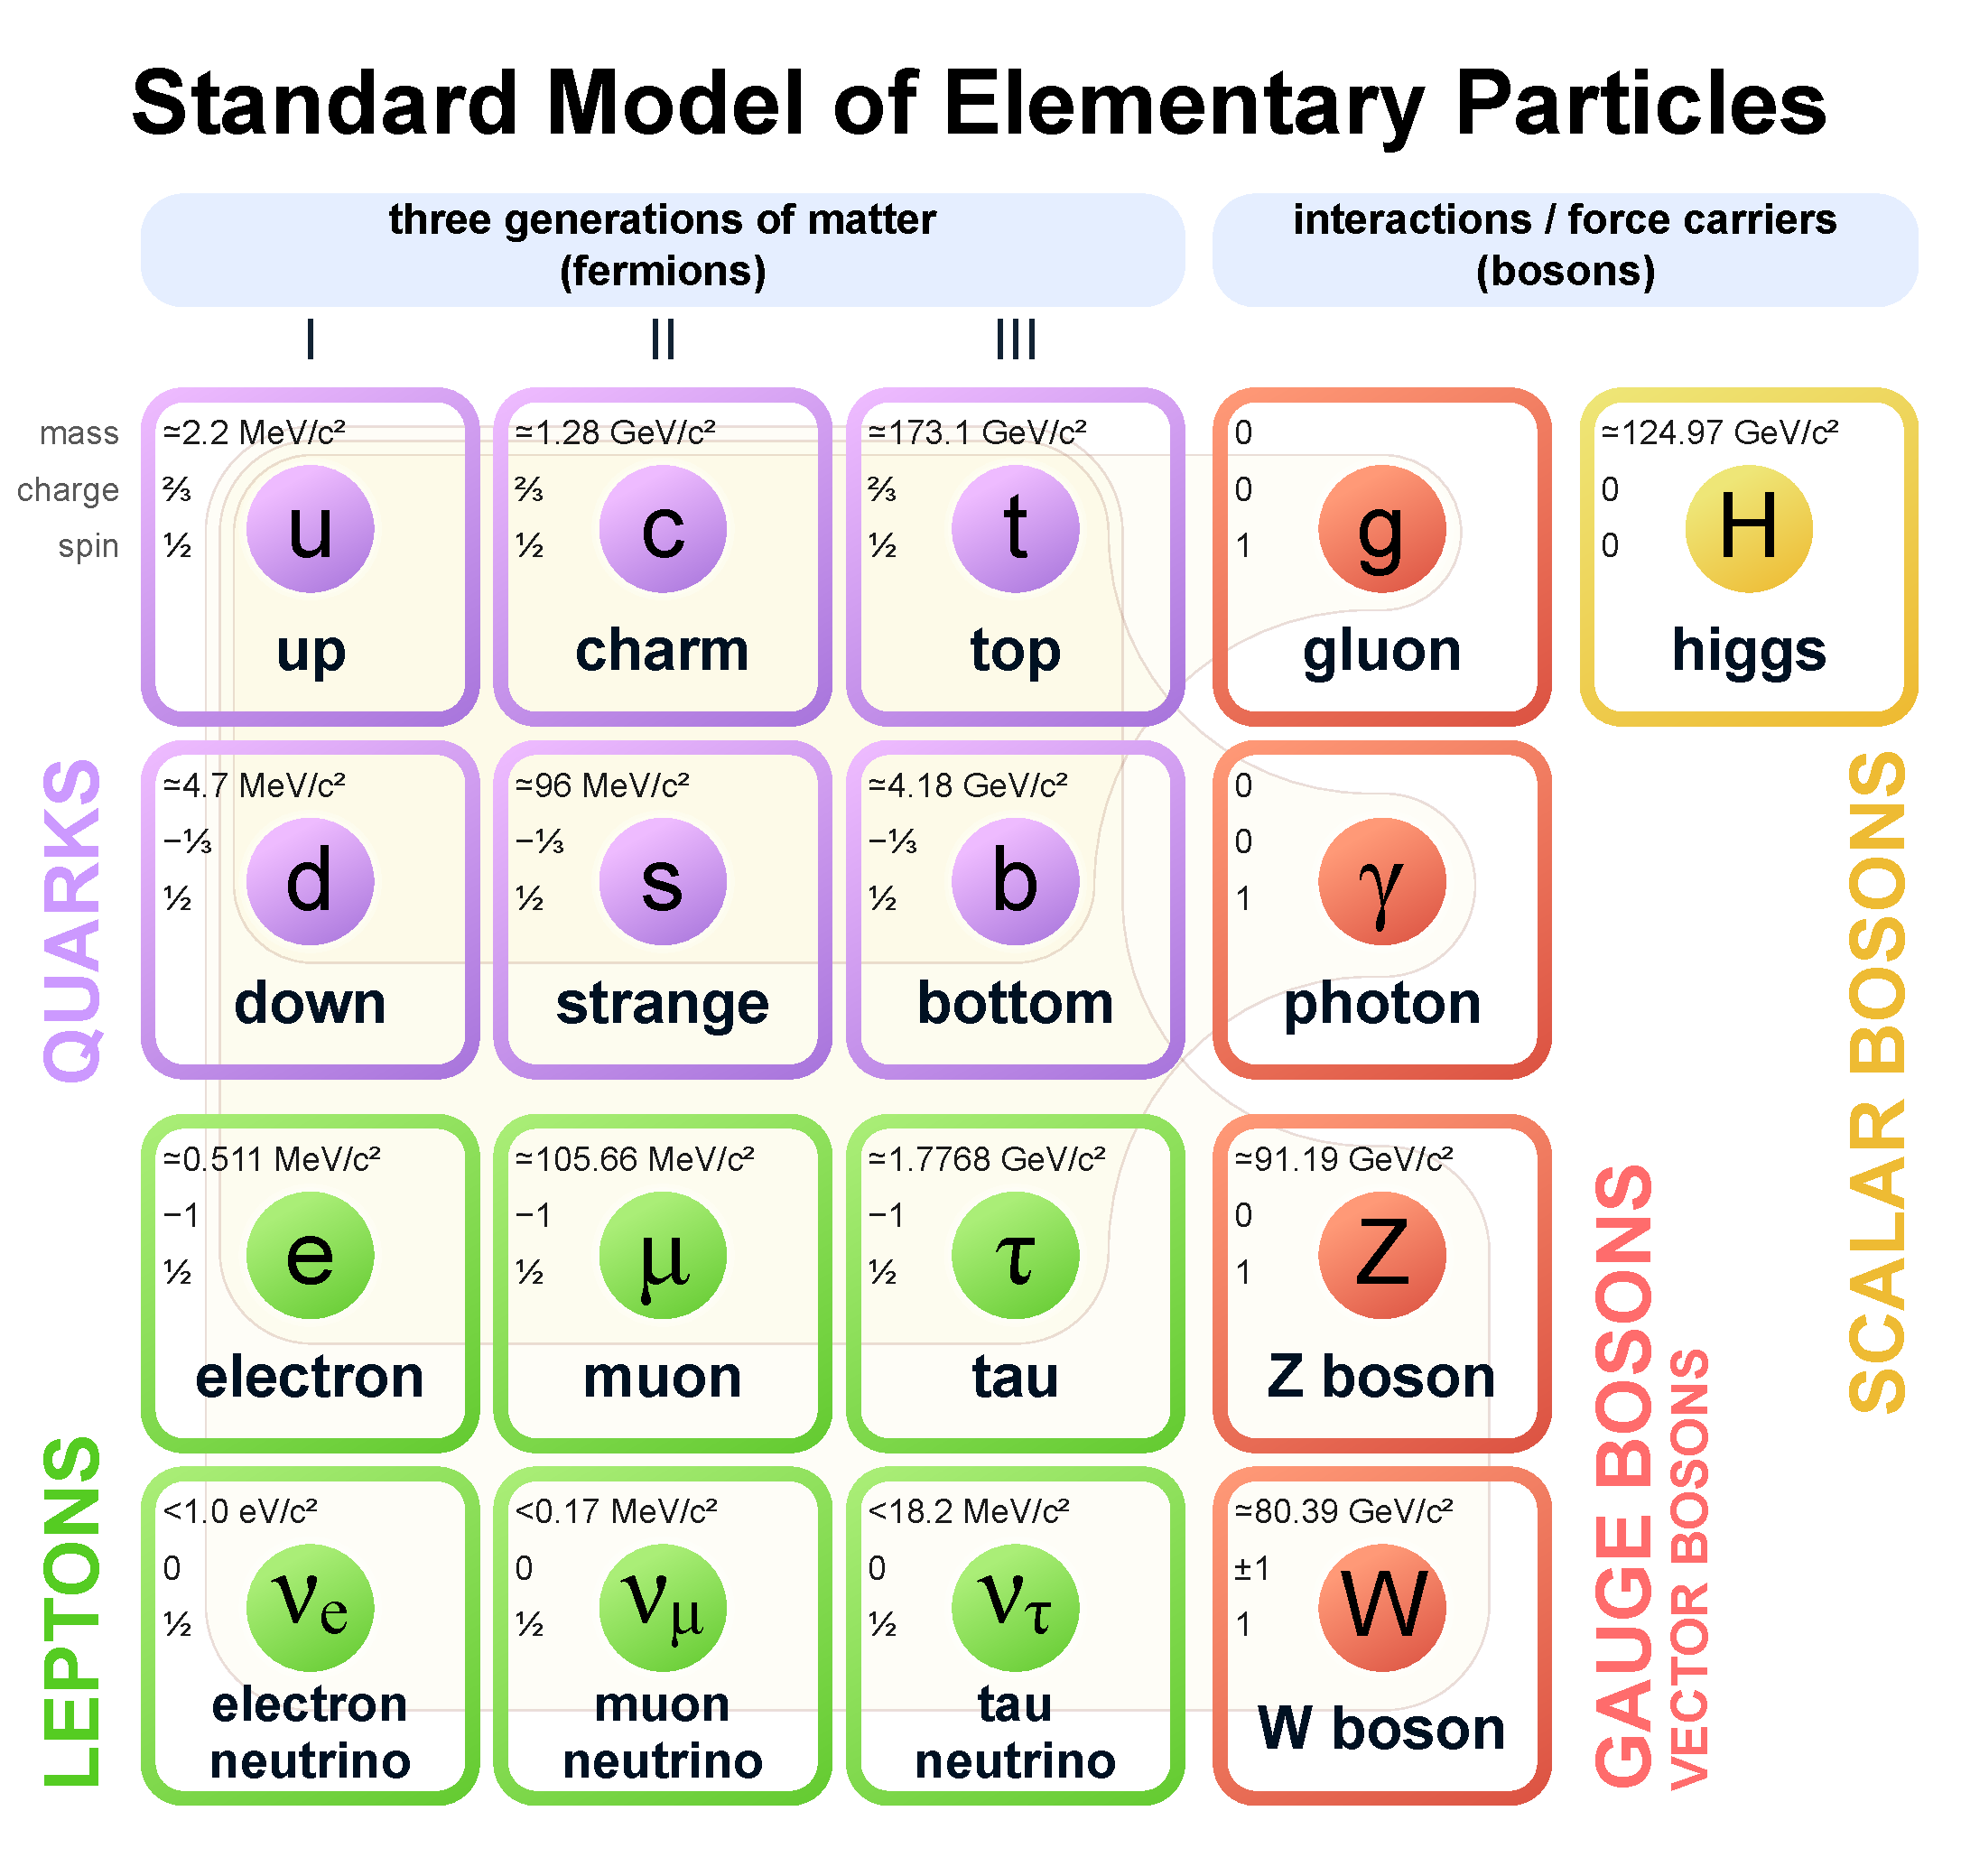
\includegraphics[width=\textwidth]{figures/Standard_Model_of_Elementary_Particles.pdf}
		\caption{\label{intro-fig:standard model}Diagram of the Standard Model of particle physics, as it currently stands. From \cite{cush_standard_2019}}
	\end{centering}
	\end{figure} 
	The 17 known particles are organized in a framework called the Standard Model of particle physics \cite{larkoski_elementary_2019-1,schwartz_quantum_2014}, displayed in schematic form in Fig.~\ref{intro-fig:standard model}.

	There are 12 particles, called \textbf{fermions}, which are the fundamental components of matter. These in turn are subdivided into \textbf{quarks} and \textbf{leptons}. Quarks, with names such as `up,' `down,' and `strange,' combine in turn to form \textbf{hadrons} --- among the hadrons are familiar composite particles like protons and neutrons. 

	The remaining 5 particles, called \textbf{bosons}, mediate interactions between particles. Four of these are responsible for three of the forces of nature: the \textbf{gluon} is responsible for the strong force; the \textbf{photon} is responsible for the electromagnetic force; and the \textbf{$W$ and $Z$ bosons} are responsible for the weak force. In terms of familiar phenomena, the strong force is what binds together the nuclei of atoms; the electromagnetic force is what makes possible most of chemistry, electronics, and modern technology; and the weak force is responsible for the decay of unstable nuclei and particles. The final boson, the \textbf{Higgs boson}, is responsible for giving mass to most of the fundamental particles, and in a technical sense is the keystone which holds the Standard Model together.

	In the Standard Model, each fermion is beholden to some subset of these bosons. The neutrinos experience the weak force and so interact via the $W$ and $Z$ bosons. The electron, muon, and tau experience the weak force as well, but they can also interact electromagnetically through exchange of photons. The quarks experience all of the fundamental forces, and can interact via any of the force-carrying bosons. It is the interaction of quarks and gluons through the strong force which will occupy most of this thesis.


\subsection{(In)completeness of the Standard Model}
	The Standard Model is a remarkable theory. It explains many observed phenomenon with unparalleled accuracy --- in fact, the Standard Model explanation of electromagnetism, called quantum electrodynamics, is the most precise physical theory ever constructed, making predictions that agree to less than 1 part per billion \cite{larkoski_elementary_2019-1}. Experiment after experiment has confirmed predictions of the Standard Model, and in this sense it is a triumph of 20th-century physics.

	In the present century, however, the strength of the theory is a significant problem in the field --- for we know that the Standard Model is incomplete. While the theory is successful at describing small-scale physics, it is not nearly as successful on a cosmic scale: it has been observed that 84.4\% of all matter in the universe is unknown to us and invisible except by gravitational signatures \cite{particle_data_group_review_2020}. We would like to understand the composition of this so-called `dark matter.' There are also more earthly hints that the Standard Model is incomplete. Among these, one of the most famous is the existence of neutrino masses. While the Standard Model describes neutrinos as massless particles, the Super-Kamiokande experiment discovered evidence in 1998 that neutrinos have a (tiny) non-zero mass \cite{super-kamiokande_collaboration_evidence_1998} --- these observations have since been verified by numerous other experiments \cite{particle_data_group_review_2020}. Finally, there are aesthetic considerations. The Standard Model, as it currently stands, has a multitude of parameters (e.g., the masses of different particles) that currently have no basis in the theory; they must be supplied externally. If possible, we would like to be able to predict these parameters eventually.\footnote{One can hardly say they understand something if, when asked why a particular detail is just so, their response is no more sophisticated than ``That's just the way it is.''}

	Thus, the Standard Model is incomplete. What can we do about that? There are two primary approaches to finding a solution:
	\begin{enumerate}
		\item \textbf{Searches for new particles:} one strategy is to design experiments that attempt to generate and detect new, previously unobserved particles. This is a well-worn technique in particle physics, responsible for many of the advances in the field over the last century. Famous examples of new-particle discoveries include the $J/\psi$ in 1974 \cite{aubert_experimental_1974,augustin_discovery_1974}, the discovery of the top quark in 1995 \cite{d0_collaboration_observation_1995,cdf_collaboration_observation_1995}, and the discovery of the Higgs boson in 2012 \cite{atlas_collaboration_observation_2012,cms_collaboration_observation_2012}. Historically, whenever new experimental frontiers have been explored, new discoveries have followed, and with them, new understanding. This is not, of course, a guarantee that such will continue in the future.\footnote{Past performance is not a guarantee of future returns.} Nevertheless, it is the underlying (if simplified) philosophy for many new particle searches at modern experiments.

		\item \textbf{Precision measurements of Standard Model parameters:} another, complementary strategy is to measure parameters of the Standard Model very precisely and then compare these measurements to theoretical predictions. These parameters could be anything from particle masses, to the strength of coupling constants, to the probability of a particular event after a particular interaction. If a discrepancy emerges, then that is a clue about where to consider modifying the Standard Model. Note, however, that to put a precise experimental measurement into a proper context, it is necessary to have at hand a precise theory. If we could measure, say, the mass of the muon\footnote{Compared to the state of the art, this would be an outrageously precise measurement. The mass of the muon is currently accepted to be \SI{105.6583745(24)}{\mega\electronvolt} \cite{particle_data_group_review_2020}, which is a precision of approximately 1 part in $10^{8}$.} to 1 part in $10^{20}$, it would do us no good if the theoretical prediction were only confident to 1 part in $10^5$. Theory and experiment must both be sufficiently advanced to take full advantage of a precise measurement.
	\end{enumerate}

	This thesis is situated firmly in the latter camp. We will be interested in precision theoretical predictions of a particular observable, called the `groomed heavy hemisphere mass,' measured in high-energy electron-positron collisions. More will be said on this topic in due time.


\subsection{Collider experiments}
	Although this thesis is theoretical in nature, it will be helpful to have some familiarity with the experiments whose outcomes we would like to predict. There is an enormous variety of experiments in particle physics, and it would be neither feasible nor helpful to discuss them all here. Instead, let us examine the two modern experiments most pertinent for our study to come. These experiments are called ATLAS (\textbf{A} large \textbf{T}oroidal \textbf{L}HC \textbf{A}pparatu\textbf{S}) and CMS (\textbf{C}ompact \textbf{M}uon \textbf{S}olenoid).\footnote{Acronyms in particle physics get very unwieldy very quickly. But look how much fun they are!} 

	Both of these are located at the Large Hadron Collider (LHC) at CERN in Geneva, Switzerland. The name of this collider is appropriate. Beams of protons are accelerated to around 99.9998\% of the speed of light using a circular ring approximately \SI{27}{\kilo\metre} in circumference.\footnote{The ring straddles the French-Swiss border.} Two beams circulate in the collider at a time, one traveling clockwise, the other counterclockwise. These beams are then maneuvered into collisions at four points around the ring, each located in the center of a massive, purpose-built experiment (in addition to ATLAS and CMS, there are two other experiments, called ALICE and LHCb). That is when the magic begins --- the collision of these protons at high energy produces, through fundamental interactions, a huge variety of particles. By observing these particles, we hope to learn something about the interactions that brought them into being.

	\begin{figure}
	\begin{center}
		\includegraphics[width=\textwidth]{figures/atlas_high_res.jpg}
		\caption{\label{intro-fig:atlas diagram}Schematic of the ATLAS experiment. For a sense of scale, note the people depicted along the bottom. Image from CERN \cite{cern_ac_layout_1998}}
	\end{center}
	\end{figure}

	ATLAS and CMS are designed as multi-purpose experiments which detect all the products of the proton-proton collisions (or at least, they try to detect them). A schematic of the ATLAS detector is displayed in Fig.~\ref{intro-fig:atlas diagram}, and a schematic of CMS is displayed in Fig.~\ref{intro-fig:cms diagram}. These detectors are built in layers surrounding the \textbf{interaction point}, with each layer serving a dedicated purpose. These layers can be summarized as follows \cite{larkoski_elementary_2019-1}:
	\begin{enumerate}
		\item In the center of each detector is the \textbf{beam pipe}. This is where collisions take place.

		\item Immediately surrounding the beam pipe is a \textbf{tracking system}. The objective of this system is to track particles as they fly away from the interaction point. From these tracks, we can glean information about the energy, charge, and type of the particles.

		\item Outside the tracking system is a \textbf{calorimetry system}. These are divided into two parts, the \textbf{electromagnetic calorimeter} and the \textbf{hadronic calorimeter}. The calorimetry system records information about the energy of particles. It works by absorbing this energy directly. The electromagnetic calorimeter is designed to most efficiently absorb particles which interact primarily through electromagnetism: electrons, photons, and the like. The hadronic calorimeter is designed to absorb hadrons like protons and neutrons.

		\item High-energy muons often escape all inner layers of the detector. Their properties are measured using \textbf{muon detectors} which line the detector's exterior.
	\end{enumerate}

	\begin{figure}
	\begin{center}
		\includegraphics[width=\textwidth]{figures/cms_160312_02.pdf}
		\caption{\label{intro-fig:cms diagram}Schematic of the CMS experiment. Note the person on the far right for scale. Image from \cite{sakuma_detector_2014}}
	\end{center}
	\end{figure}

	Using these systems, ATLAS and CMS are able to measure the results of more than a billion collision events per second, though the data is rapidly processed through a \textbf{triggering} system to reduce stored data rates to the \si{\kilo\hertz} level. \cite{atlas_outreach_atlas_2012,atlas_collaboration_performance_2017}. This data gets stored and processed at data centers distributed globally.\footnote{The scale of ATLAS and CMS is absolutely mind-boggling.} Typical searches and measurements at these experiments then look for statistical signatures of interesting physics. This could be anything from an unexpected excess of events in a particular region of phase space (for a particle search) to the probability distribution of observing particular values of particle parameters (for Standard Model measurements). 


\section{Thesis goals}
	The objectives of this thesis can be divided into two categories: scientific and pedagogical. It will be necessary to properly balance the two. Our scientific focus will be rather technical, and too much emphasis on this would cloud the narrative and make it difficult to learn from the work. The other side of this coin is that, to achieve the pedagogical goals of the thesis, we will have to complete only a partial calculation. This is not a complete loss --- what we achieve will be meaningful in its own right, and we will not have to suffer unnecessary tedium. Nevertheless, I warn the reader in advance that the story will be left incomplete.

	But enough digression --- what are the goals?

\subsection{Scientific}
	The primary scientific objective of the thesis will be to complete an all-orders calculation of the distribution of groomed heavy hemisphere mass in $e^+ e^- \to \text{jets}$ events, in the limit that the jet mass is approximately equal to the grooming cutoff. There are several moving parts here:
	\begin{enumerate}
		\item \textbf{$e^+ e^- \to \text{jets}$ events:} We are going to consider collider events in which electron and positrons annihilate to produce quarks and gluons. At high energies, because of the nature of the strong force, quarks and gluons manifest themselves in a detector as \textbf{jets}, or collimated sprays of hadronic particles. Note that these are not the type of collision events observed at the LHC, which is a proton-proton collider. Electron-positron annihilation is much easier to handle theoretically, and it turns out that we could, in principle, generalize our results to $pp$ collisions without much difficulty.

		\item \textbf{Heavy hemisphere mass:} We are interested in an observable called heavy hemisphere mass. To compute heavy hemisphere mass, one can divide a collision event into two hemispheres, measure the mass of both hemispheres, and then take the greater of the two masses.

		\item \textbf{Groomed:} When measuring an observable like jet mass, modern experiments like ATLAS and CMS must take into account significant amounts of background radiation from simultaneous events in the detector. One common technique to manage this background is to perform `jet grooming,' in which undesirable radiation is algorithmically removed from a jet. We will consider a particular grooming algorithm called the Modified Mass Drop Tagger (mMDT) \cite{dasgupta_towards_2013}, in which radiation with energy below some threshold is ignored. Such grooming can significantly alter the distribution of an observable, and it has important experimental and theoretical advantages. Understanding the effect of grooming on observables like jet mass is an active area of research.

		\item \textbf{The limit:} Jets are a phenomenon of the strong force, and the theory of the strong force is rather unwieldy. It is therefore difficult to accurately predict an entire observable distribution with only one calculation. While the distribution of groomed heavy hemisphere mass is well understood in the low-mass limit \cite{kardos_groomed_2020,kardos_two-_2020,frye_factorization_2016} and in the high-mass regime \cite{kardos_soft-drop_2018}, little study has been performed in the regime where the mass is approximately equal to the mMDT energy cutoff. Nevertheless, interesting physics occurs in this region --- whereas events throughout the distribution all rely on the production of two back-to-back quarks, this region is the one in which a third (gluon) emission just begins to be resolved above the grooming threshold. Thus, this region is our focus.

		\item \textbf{Calculation:} Just as we must perform calculations in particular limits to work with the strong force, so we must also perform calculations perturbatively, as a series expansion in the strong coupling constant $\alpha_s$. That is, if we want to compute an observable $\omega$, it is not usually feasible\footnote{At least with current theoretical techniques.} to do so with perfect precision. Instead, we can expand $\omega$ in $\alpha_s$,
		\begin{equation}
			\omega(\alpha_s) = \omega_0 + \omega_1 \alpha_s + \omega_2 \alpha_s^2 + \dots = \sum_{n = 0}^\infty \omega_n \alpha_s^n.
		\end{equation}
		Then, to compute $\omega$ to a particular desired accuracy, we can simply compute the coefficients $\omega_i$ up to a particular order in $\alpha_s$. Unfortunately, $\alpha_s$ is not a particularly small quantity, taking a value of order $0.1$.\footnote{The strong coupling constant is not actually a constant\dots\, it changes with the energy of observation. This process is called the \textbf{running} of the strong coupling \cite{larkoski_elementary_2019-1}. At the mass of the $Z$ boson, $\alpha_s(m_Z) = 0.1179(10)$ \cite{particle_data_group_review_2020}.} This means it often takes several terms to obtain a reasonable degree of accuracy.

		\item \textbf{All-orders:} That said, we are aiming to achieve an all-orders calculation of the groomed heavy hemisphere mass. This does \textit{not} mean that we will determine the distribution to infinite precision (i.e., infinite order in $\alpha_s$). Instead, it means that we will derive an expression which can be used to push to \textit{arbitrary accuracy} in $\alpha_s$, given the proper accuracy of inputs (and the proper degree of mathematical sophistication). Thus, by an `all-orders calculation,' we mean that we will develop a \textit{framework} for achieving precision results. The term `all-orders' also refers to the fact that our calculation will account for the influence of large logarithms at every order in $\alpha_s$ through the process of resummation.
	\end{enumerate}
	A more complete development of these foundational concepts will be provided in Chapter \ref{chap:technical}.


\subsection{Pedagogical}
	The primary pedagogical goal of this thesis is to understand the inner workings of a particular class of precision calculations in modern high-energy physics. The scientific objectives described above require a set of advanced theoretical tools which are interesting in their own right, but difficult to understand except through examples and context. Such tools include:
	\begin{enumerate}
		\item \textbf{Dimensional regularization:} There will be times when we must evaluate an integral which diverges when computed in the usual 4 dimensions (3 spatial dimensions and one temporal). We will get around this problem by performing such calculations in $d = 4 - 2\epsilon$ dimensions for some small $\epsilon$ \cite{schwartz_quantum_2014}. The result will still diverge if we send $\epsilon \to 0$, but operating in this way will allow us to see the divergences explicitly, and cancel them as appropriate.

		\item \textbf{Resummation:} A na\"ive series expansion of the distribution which we want to compute is plagued by corrections that take the form of logarithms of ratios of differing energy scales (e.g., the energy scale of a jet versus the energy scale of background radiation). When these scales are sufficiently different, the logarithm of their ratio becomes very large. Resummation is the process of getting a theoretical handle on these logarithmic corrections \cite{larkoski_elementary_2019-1}. The primary thrust of this thesis can be viewed, in a sense, as one large resummation calculation.

		\item \textbf{Soft and collinear effective theory (SCET):} Quantum field theory (QFT) is a remarkable description of the (subatomic) universe, but for our purposes it is too much machinery. Instead of using the full theory, we will make use of a low-energy effective theory called Soft-Collinear Effective Theory (SCET). SCET is essentially a limiting case of full QFT, useful in the regime which we will occupy ourselves. As a simpler theory, SCET has some useful properties that we will exploit.
	\end{enumerate}


\section{Technical and notational conventions}
	Before we embark, we must lay some mathematical ground rules. First, we hold Planck's constant and the speed of light to be equal to unity: $\hbar = c = 1$. It turns out that non-unity values of these quantities are, for our purposes, redundant; when converting a given quantity back to SI units, the appropriate factors of $c$ and $\hbar$ can be intuited from context. The result is that all quantities will be measured in units of energy. 

	Physics where we will be working is at the \si{\giga\electronvolt} scale and higher. Therefore, to a high degree of accuracy, we will assume all particles to be massless.

	Unless otherwise stated (and we \textit{will} eventually state otherwise), we will work in $4$ dimensions, comprising the usual three spatial dimensions and one temporal dimension. Vectors in $4$ dimensions (called four-vectors) are denoted by a Greek-letter index and take the form
	\begin{equation}
		p^\mu = (p^0, p^1, p^2, p^3).
	\end{equation}
	The $0$-th component of a four-vector is its `time' (or equivalent) component, and the others are the `spatial' (or equivalent) components. Thus, for example, a four-vector representing position would be
	\begin{equation}
		x^\mu = (t, x, y, z),
	\end{equation}
	while a four-momentum has the components
	\begin{equation}
		p^\mu = (E, p_x, p_y, p_z)
	\end{equation}
	with energy taking the place of time. It is sometimes convenient to refer to lower-dimensional pieces of a four-vector (usually two or three of the spatial components). When doing so, we will denote the sub-vector using a bold-face letter:
	\begin{equation}
		p^\mu = (E, \vb{p}), \quad \vb{p} = (p_x, p_y, p_z).
	\end{equation}

	As is standard in high-energy physics, we will neglect the effects of gravity and assume we are working in a flat space-time. When combining four-vectors, we will therefore use the `mostly minus' metric\footnote{Also known as the `West Coast' metric, among other names. The `East Coast' metric takes the opposite sign convention. Our convention here is clearly the correct one, as it results in naturally positive masses.}
	\begin{equation}
		\eta^{\mu \nu} = \begin{pmatrix}
			1 & 0 & 0 & 0 \\
			0 & -1 & 0 & 0 \\
			0 & 0 & -1 & 0 \\
			0 & 0 & 0 & -1
		\end{pmatrix}.
	\end{equation}
	We will also employ the Einstein summation notation, in which one sums over repeated indices in an expression (known as `contracting' the index). Hence, for $p^\mu = (p^0, \vb{p})$ and $k_\mu = (k_0, \vb{k})$, we have
	\begin{equation}
		k_\mu p^\mu = k_0 p^0 + k_1 p^1 + k_2 p^2 + k_3 p^3.
	\end{equation}

	With our choice of metric, there is little mechanical difference between a contravariant and a covariant four-vector; one picks up a formal minus sign in the spatial components, but that is all. We will, therefore, not distinguish between the two, and we will interchange upper and lower indices freely, bearing in mind that contracting an index negates the spatial terms of the sum. Hence, for $p^\mu = (p^0, \vb{p})$ and $k^\mu = (k^0, \vb{k})$, we will write\footnote{Sorry, Joel.}
	\begin{equation}
		k^\mu p_\mu = k_\mu p^\mu = k^\mu p^\mu = k_\mu p_\mu = k^0 p^0 - \vb{k} \cdot \vb{p}.
	\end{equation}
	The final term is the standard dot product between the three-vectors. This choice enables us to abuse notation in a convenient manner: we will often drop the Greek sub/superscript on four-vectors, and use the standard notation of linear algebra to indicate their contraction:
	\begin{equation}
		k \cdot p = k^0 p^0 - \vb{k}\cdot\vb{p}.
	\end{equation}

	Let us end with a reminder about the connection between these four-vectors and the physical world. Suppose a particle has a momentum four-vector $p^\mu$. Transforming our frame of reference to the particle's rest frame, we could write $p^\mu = (E, 0, 0, 0)$, where $E$ is the particle's energy. But then, recalling the famous relation $E = mc^2 = m$ (since we set $c = 1$), we have
	\begin{equation}
		p^2 = p \cdot p = E^2 = m^2.
	\end{equation}
	Thus, the square of a particle's four-momentum yields its squared mass. Recall now that we are assuming all particles to be massless; therefore, for any `on-shell' particle (that is, a particle that could exist on its own and not just in some quantum fluctuation), we see that $p^2 = 0$, and also that $E^2 = \vb{p} \cdot \vb{p}$.\footnote{This is not strictly an accurate proof of these properties, since massless particles move at the speed of light and one cannot boost into a light-like reference frame using Lorentz transformations. But the spirit of the argument is right, and the result is the same regardless.} This will greatly simplify our calculations later on.

	With these details out of the way, let us proceed.

% \ifstandalone
% \bibliographystyle{../bsts/myJHEP} 
% \bibliography{../jet_substructure}
% \fi
\end{document}


	

\chapter{QCD, jet grooming, and our toolbox}\label{test}
	
	First chapter here

	\section{Quantum Chromodynamics (QCD)}
	\subsection{Cross sections}

	\subsection{Fermi's golden rule}

	\subsection{Running coupling}

	\section{Jets}

	\section{mMDT Grooming}

	\section{Soft Collinear Effective Theory (SCET)}

	\section{Dimensional regularization}

	\section{Resummation}


\chapter{Leading-order calculation}

	% This is the Reed College LaTeX thesis template. Most of the work 
% for the document class was done by Sam Noble (SN), as well as this
% template. Later comments etc. by Ben Salzberg (BTS). Additional
% restructuring and APA support by Jess Youngberg (JY).
% Your comments and suggestions are more than welcome; please email
% them to cus@reed.edu
%
% See http://web.reed.edu/cis/help/latex.html for help. There are a 
% great bunch of help pages there, with notes on
% getting started, bibtex, etc. Go there and read it if you're not
% already familiar with LaTeX.
%
% Any line that starts with a percent symbol is a comment. 
% They won't show up in the document, and are useful for notes 
% to yourself and explaining commands. 
% Commenting also removes a line from the document; 
% very handy for troubleshooting problems. -BTS

% As far as I know, this follows the requirements laid out in 
% the 2002-2003 Senior Handbook. Ask a librarian to check the 
% document before binding. -SN

%%
%% Preamble
%%
% \documentclass{<something>} must begin each LaTeX document
\providecommand{\main}{..}
\documentclass[12pt,twoside,class=../reedthesis, crop=false]{standalone}
% Packages are extensions to the basic LaTeX functions. Whatever you
% want to typeset, there is probably a package out there for it.
% Chemistry (chemtex), screenplays, you name it.
% Check out CTAN to see: http://www.ctan.org/
%%
\usepackage{graphicx,latexsym} 
\usepackage{amssymb,amsthm,amsmath}
\usepackage{longtable,booktabs,setspace} 
\usepackage{chemarr} %% Useful for one reaction arrow, useless if you're not a chem major
\usepackage[hyphens]{url}
\usepackage{rotating}
\usepackage{hyperref}

\usepackage{physics}
\usepackage{siunitx}
\usepackage{xcolor}

\usepackage{tikz-feynman}
% \usepackage{standalone}
% \usepackage{natbib}
% Comment out the natbib line above and uncomment the following two lines to use the new 
% biblatex-chicago style, for Chicago A. Also make some changes at the end where the 
% bibliography is included. 
%\usepackage{biblatex-chicago}
%\bibliography{thesis}

% \usepackage{times} % other fonts are available like times, bookman, charter, palatino

\providecommand{\zcut}{z_\mathrm{{cut}}}
\providecommand{\LIPS}{\mathrm{LIPS}}

\providecommand{\cM}{\mathcal{M}}
\providecommand{\cO}{\mathcal{O}}


\setlength{\parskip}{0pt}
%%
%% End Preamble
%%
%% The fun begins:
\begin{document}
	In order to develop an intuition for the mathematical tools we will put to use in the all-orders calculation of groomed heavy hemisphere mass, let us first compute the first-order (or rather, first \textit{nontrivial} order) distribution of the observable. A simple electron-positron production with the production of two quark jets, $e^+ e^- \to q\bar q$, would produce a constant distribution: the mass of the heavy hemisphere would simply be half of the final mass. The lowest-order nontrivial distribution corresponds to an $e^+ e^- \to q\bar q g$ event, in which an electron and positron annihilate to produce a quark-antiquark pair, off of which a single gluon is emitted. The location of the gluon in phase space sets the heavy hemisphere mass. This process is depicted in a Feynman diagram in Fig.~\ref{fig:first-order diagram}.

	\begin{figure}
	\begin{center}
		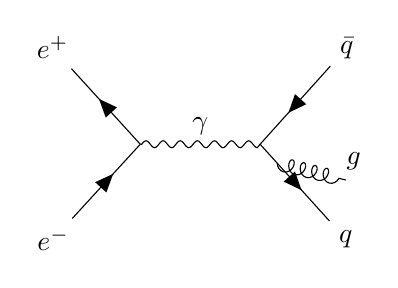
\begin{tikzpicture}
		\begin{feynman}
			\diagram [horizontal=a to b] {
  				i1 [particle=\(e^{-}\)] -- [fermion] a -- [fermion] i2 [particle=\(e^{+}\)],
  				a -- [photon, edge label=\(\gamma\)] b,
  				f1 [particle=\(\bar q\)] -- [fermion] b -- [fermion] f2 [particle=\(q\)],
			};

			\vertex [above = 0.75cm of f2] (r);
			\vertex [right = 0.1cm of r, label = $g$] (g);
    		\draw [gluon] ($(f2)!0.8!(b)$) -- (r);
		\end{feynman}
		\end{tikzpicture}

		\caption{\label{fig:first-order diagram}Feynman diagram of an $e^+ e^- \to q\bar q g$ event.}
	\end{center}
	\end{figure}

	We will work in the limit that the heavy hemisphere mass $\rho$ is approximately equal to the mMDT cutoff $\zcut$, which is itself small: $\rho \sim \zcut \ll 1$. We will utilize the strategy of regions \cite{becher_introduction_2015-1} to compute the distribution. This is necessary because the distribution is essentially singular in the limit of interest {\color{red}\textbf{[TODO: is this accurate?]}}. The method of regions entails computing the distribution in all singular regions of phase space, then summing the results at the end to generate the full distribution.\footnote{The fact that this works is rather magical.} There are three singular regions of phase space:
	\begin{enumerate}
		\item The \textbf{soft region}, in which the gluon is emitted with low energy.

		\item The \textbf{collinear region}, in which the gluon is emitted collinear to the quark or antiquark.

		\item The \textbf{soft-collinear region}, in which the gluon is both low-energy and collinear to the quark or antiquark. This region is covered by both the soft and the collinear calculations, so we must subtract it away to avoid double-counting.
	\end{enumerate}
	If we label these cross sections $\sigma_\text{soft}$, $\sigma_\text{collinear}$, and $\sigma_\text{soft-collinear}$, respectively, then the full cross distribution will be
	\begin{equation}
		\frac{d\sigma}{d\rho} = \frac{d\sigma_\text{soft}}{d\rho} + \frac{d\sigma_\text{collinear}}{d\rho} + \frac{d\sigma_\text{soft-collinear}}{d\rho}.
	\end{equation}
	Let us calculate these components now.

\section{Soft gluon}
\subsection{Setup}
	For now, we assume a soft (i.e., low-energy) gluon. Recall that the (normalized) heavy hemisphere mass is defined to be
	\begin{equation}
		\rho = \qty(\frac{m_h}{E_h})^2
	\end{equation}
	with $m_h$ the mass of the more massive hemisphere and $E_h$ its energy.

	We first need to sort out the kinematics of the event. Let us shift our reference frame so that the quark has momentum
	\begin{equation}
		p_1^\mu = \frac{Q_q}{2}\qty(1, 0, 0, 1)
	\end{equation}
	and the antiquark has momentum
	\begin{equation}
		p_2^\mu = \frac{Q_q}{2}\qty(1, 0, 0, -1),
	\end{equation}
	and let the gluon have momentum $k^\mu$. The soft-gluon limit means that the energy of the gluon is $k^0 \ll 1$. In this case, the quarks carry most of the energy, so we can approximate $Q_q \approx Q$, the total energy of the event. Furthermore, let us assume that the gluon is emitted in the hemisphere containing the quark (the problem is symmetric under quark-antiquark exchange, so we will simply multiply the cross section by $2$ at the end to account for this assumption). Then the momentum of the heavy hemisphere is
	\begin{equation}
		p_h = p_1 + k,
	\end{equation}
	so the heavy hemisphere has mass
	\begin{equation}
	\begin{aligned}
		m_h^2 &= p_h^2 = \qty(p_{1, 0} + k_0)^2 - (k_1)^2 - (k_2)^2 - (p_{1, 3} + k_3)^2 \\
		&= 2p_{1, 0}k_0 - 2p_{1, 3}k_3 + p_1^2 + k^2 \\
		&= Q(k_0 - k_3).
	\end{aligned}
	\end{equation}
	The last line follows because we assume every particle to be massless, such that $p_1^2 = k^2 = 0$.\footnote{This is a reasonably accurate assumption for the energies accessible by colliders, and makes our calculations much easier. The gluon is actually massless regardless of the theoretical assumptions made.} Now let us introduce the \textbf{light-cone coordinates}
	\begin{align}
		k^+ &\equiv k^0 - k^3 & k^- &\equiv k^0 + k^3,
	\end{align}
	this can be written simply as
	\begin{equation}
		m_h^2 = Q k^+.
	\end{equation}
	The energy of the heavy hemisphere is
	\begin{equation}
		E_h = p_{1, 0} + k_0 = \frac{Q}{2} + k_0 \approx \frac{Q}{2},
	\end{equation}
	since, for a soft gluon, $k_0 \ll Q/2$. The heavy hemisphere mass is therefore
	\begin{equation}\label{eq:soft mass}
		\rho = \frac{Q k^+}{Q^2 / 4} = \frac{4k^+}{Q}.
	\end{equation}
	This means that we will need to insert the measurement function
	\begin{equation}
		\delta\qty(\rho - \frac{4k^+}{Q})
	\end{equation}
	into Fermi's Golden Rule.

	With the kinematics under our belt, let us think about the effects of an mMDT groomer. For the simple case of only 3 particles, the groomer only keeps pairs of particles $i$ and $j$ for which \cite{dasgupta_towards_2013,kardos_two-_2020}
	\begin{equation}
		\frac{\min\qty[E_i, E_j]}{E_i + E_j} > \zcut.
	\end{equation}
	This must be true for the quark and gluon; since the gluon has lower energy then the quark, this necessitates that
	\begin{equation}
		\frac{k_0}{E_h} = \frac{(k^+ + k^-)/2}{Q/2} > \zcut,
	\end{equation}
	or
	\begin{equation}\label{eq:soft grooming}
		k^+ + k^- > Q\,\zcut.
	\end{equation}
	Moreover, since we are assuming that the gluon shares a hemisphere with the quark, we must also have $k_3 > 0$, which requires
	\begin{equation}\label{eq:gluon quark hemisphere}
		k^- - k^+ > 0.
	\end{equation}
	Equations \ref{eq:soft grooming} and \ref{eq:gluon quark hemisphere} generate the phase space constraints
	\begin{equation}
		\Theta\qty(k^+ + k^- - Q\,\zcut)\Theta\qty(k^- - k^+).
	\end{equation}
	When we insert these into Fermi's Golden Rule, the differential cross section takes the form
	\begin{equation}\label{eq:soft cross section preliminary}
		\frac{d\sigma_{\text{soft}}}{d\rho} = 2\int d\LIPS\,\abs{\cM}^2 \delta\qty(\rho - \frac{4k^+}{Q}) \Theta\qty(k^+ + k^- - Q\,\zcut)\Theta\qty(k^- - k^+).
	\end{equation}
	Here, $d\LIPS$ is a differential element of Lorentz-invariant phase space, and $\cM$ is the matrix element governing the $e^+ e^- \to q\bar q g$ process.

	Assuming a soft gluon, the matrix element is well-known in the literature (see Eqs.\ 87 and 88 of \cite{catani_infrared_2000}):
	\begin{equation}
		\abs{\cM}^2 = 4\pi \alpha_s \sigma_0 C_F \mu^{2\epsilon} \frac{p_1 \cdot p_2}{(p_1 \cdot k)(p_2 \cdot k)}.
	\end{equation}
	Here, $\alpha_s$ is the strong coupling constant\footnote{Which is not really a constant}, $\sigma_0$ is the cross section for $e^+ e^- \to q\bar q$, $C_F$ is the quadratic Casimir of the fundamental representation of color (taken to be $C_F = 4/3$ for our purposes \cite{particle_data_group_review_2020}), and $\mu$ is a mass scale introduced to ensure that the differential cross section will remain dimensionless in $d = 4 - 2\epsilon$ dimensions. Inserting the values of $p_1$, $p_2$, and $k$, we have
	\begin{equation}\label{eq:soft matrix element}
		\abs{\cM}^2 = 4\pi \alpha_s \sigma_0 C_F \mu^{2\epsilon} \frac{2}{k^+ k^-}.
	\end{equation}

	Now we must unpack the Lorentz-invariant phase space element $d\LIPS$. Working in $d$ dimensions, the standard form is
	\begin{equation}
		d\LIPS = \frac{d^d k}{(2\pi)^{d-1}}\delta(k^2)\Theta(k_0),
	\end{equation}
	where the Dirac delta and Heaviside functions ensure that the gluon is on-shell (i.e., real) with positive energy. If $\epsilon = 0$, we would have
	\begin{equation}
		d^d k = d^4 k = dk_0 \,dk_1 \,dk_2 \,dk_3.
	\end{equation}
	When we transform to light-cone coordinates with $(k_0, k_3) \to (k^+, k^-)$, the Jacobian of the transformation is
	\begin{equation}
		\frac{\partial(k_0, k_3)}{\partial(k^+, k^-)} = \mqty(1/2 & 1/2 \\ -1/2 & 1/2),
	\end{equation}
	so
	\begin{equation}
		dk_0 \, dk_3 = \abs{\det \frac{\partial(k_0, k_3)}{\partial(k^+, k^-)}} dk^+ dk^- = \frac{1}{2} dk^+ dk^-.
	\end{equation}
	Now let $k_\perp = (k_1, k_2)$ be the transverse components of the gluon momentum. For $\epsilon \neq 0$, we imagine that these transverse components are the ones which bleed into the modified dimensions. Therefore, after noticing that
	\begin{equation}
		\delta(k^2) = \delta(k_0^2 - k_3^3 - k_\perp^2) = \delta(k^+ k^- - k_\perp^2),
	\end{equation}
	we have
	\begin{equation}
		d\LIPS = \frac{dk^+ dk^- d^{d-2}k_\perp}{2(2\pi)^{d-1}} \delta(k^+ k^- - k_\perp^2)\Theta(k^+ + k^-).
	\end{equation}
	Now it is convenient to transfer the $2 - 2\epsilon$ dimensions of $k_\perp$ into spherical coordinates, so that
	\begin{equation}
		d^{d - 2}k_\perp = k_\perp^{d-3} dk_\perp d\Omega_{d-2}
	\end{equation}
	with $\Omega_{d-2}$ the solid angle of the $(d-2)$-dimensional unit sphere. Since none of the terms in the cross section of Eq.~\ref{eq:soft cross section preliminary} or matrix element of Eq.~\ref{eq:soft matrix element} have angular dependence, we can go ahead and integrate the solid angle:
	\begin{equation}
		\int d\Omega_{d-2} = \frac{2\pi^{(d-2)/2}}{\Gamma(\frac{d-2}{2})}
	\end{equation}
	with $\Gamma(x)$ the gamma function; this identity comes from Eq.\ B.28 of \cite{schwartz_quantum_2014}.
	Therefore,
	\begin{equation}
		d\LIPS = \frac{2\pi^{(d-2)/2}}{\Gamma(\frac{d-2}{2})} \frac{dk^+ dk^- dk_\perp}{2(2\pi)^{d-1}} k_\perp^{d-3} \delta(k^+ k^- - k_\perp^2)\Theta(k^+ + k^-).
	\end{equation}
	As a final step, we can resolve this delta function:
	\begin{equation}
		\delta(k^+ k^- - k_\perp^2) = \frac{1}{\sqrt{k^+ k^-}}\,\delta\qty(k_\perp - \sqrt{k^+ k^-}).
	\end{equation}
	Then integrating over $k_\perp$ yields
	\begin{equation}
		\int dk_\perp \frac{k_\perp^{d-3}}{2\sqrt{k^+ k^-}}\,\delta\qty(k_\perp - \sqrt{k^+ k^-}) = \qty(k^+ k^-)^{(d-4)/2}.
	\end{equation}
	Putting everything together, inserting $d = 4 - 2\epsilon$, and simplifying, we are left with
	\begin{equation}
		d\LIPS = \frac{(4\pi)^{\epsilon}}{\Gamma(1-\epsilon)8\pi^2}\frac{dk^+ dk^-}{(k^+ k^-)^\epsilon} \Theta(k^+ + k^-).
	\end{equation}
	Notice that a factor of $(k^+ k^-)^\epsilon$ has been introduced --- this is what will help us capture divergences as we work and cancel them at the end. Finally, we will work using a convention known as \textbf{modified minimal subtraction}, under which we will throw away factors of $(4\pi)^\epsilon$ and set the Euler-Mascheroni constant to be $\gamma_E \to 0$ when it appears (this does not affect the final result, but will make calculations slightly less unwieldy). Under this scheme, we have
	\begin{equation}\label{eq:soft phase space}
		d\LIPS = \frac{1}{\Gamma(1-\epsilon)8\pi^2}\frac{dk^+ dk^-}{(k^+ k^-)^\epsilon} \Theta(k^+ + k^-).
	\end{equation}
	as our final phase space element.

	Combining Eqs.~\ref{eq:soft cross section preliminary}, \ref{eq:soft matrix element}, and \ref{eq:soft phase space} then yields the full cross section:
	\begin{equation}\label{eq:soft cross section integral}
	\boxed{
	\begin{aligned}
		\frac{1}{4\pi\alpha_s\sigma_0 C_F}\frac{d\sigma_{\text{soft}}}{d\rho} = \frac{\mu^{2\epsilon}}{\Gamma(1-\epsilon)2\pi^2}\int &\frac{dk^+ dk^-}{(k^+ k^-)^{1+\epsilon}} \delta\qty(\rho - \frac{4k^+}{Q}) \Theta(k^+ + k^-) \\
		&\times \Theta\qty(k^+ + k^- - Q\,\zcut)\Theta\qty(k^- - k^+).
	\end{aligned}
	}
	\end{equation}

\subsection{Calculation}
	The integral of Eq.~\ref{eq:soft cross section integral} is relatively straightforward to evaluate. The first step is to resolve the Dirac delta:
	\begin{equation}
		\delta\qty(\rho - \frac{4k^+}{Q}) = \frac{Q}{4}\delta\qty(k^+ - \frac{Q\rho}{4}).
	\end{equation}
	The integrating over $k^+$ yields
	\begin{equation}
	\begin{aligned}
		\frac{1}{4\pi\alpha_s\sigma_0 C_F}\frac{d\sigma_{\text{soft}}}{d\rho} = \frac{\mu^{2\epsilon}}{\Gamma(1-\epsilon)2\pi^2} \frac{1}{\rho} &\qty(\frac{4}{Q\rho})^{\epsilon} \int \frac{dk^- }{(k^-)^{1+\epsilon}}\Theta\qty(\frac{Q \rho}{4} + k^-)  \\
		&\times \Theta\qty(\frac{Q\rho}{4} + k^- - Q\,\zcut)\Theta\qty(k^- - \frac{Q\rho}{4}).
	\end{aligned}
	\end{equation}
	Now, the integrand is only non-zero when
	\begin{align}
		k^- &> -\frac{Q\rho}{4} & k^- &> Q\qty(\zcut - \frac{\rho}{4}) & k^- &> \frac{Q\rho}{4}.
	\end{align}
	If the second and third requirements are satisfied, then so is the first, so we can ignore it. To deal with the others, notice that each is stricter for different values of $\rho$: if $\rho < 2\zcut$, then
	\begin{equation}
		Q\qty(\zcut - \frac{\rho}{4}) > \frac{Q\rho}{4},
	\end{equation}
	and the opposite is true if $\rho > 2\zcut$. We can therefore break the integral into two pieces:
	\begin{equation}
	\begin{aligned}
		\int \frac{dk^- }{(k^-)^{1+\epsilon}}&\Theta\qty(\frac{Q \rho}{4} + k^-) \Theta\qty(\frac{Q\rho}{4} + k^- - Q\,\zcut)\Theta\qty(k^- - \frac{Q\rho}{4}) \\
		&= \Theta\qty(\rho - 2\zcut) \int_{Q\rho/4}^\infty \frac{dk^-}{(k^-)^{1+\epsilon}} + \Theta(2\zcut - \rho) \int_{Q(z - \rho/4)}^\infty \frac{dk^-}{(k^-)^{1+\epsilon}}.
	\end{aligned}
	\end{equation}
	If we take $\epsilon > 0$, then these integrals yield a finite result:
	\begin{equation}
	\begin{aligned}
		\frac{1}{4\pi\alpha_s\sigma_0 C_F}\frac{d\sigma_{\text{soft}}}{d\rho} = \frac{\mu^{2\epsilon}}{\Gamma(1-\epsilon)2\pi^2} \frac{1}{\rho} &\qty(\frac{4}{Q\rho})^{\epsilon} \frac{1}{\epsilon}\Bigg[\Theta(\rho - 2\zcut)\qty(\frac{Q\rho}{4})^{-\epsilon} \\
			&\hspace{1cm}+ \Theta(2\zcut - \rho)\qty(Q\qty(\zcut - \frac{\rho}{4}))^{-\epsilon}\Bigg].
	\end{aligned}
	\end{equation}
	Notice how dimensional regularization helped us achieve this calculation: without the regulating $(k^-)^\epsilon$, the integrals would have diverged without an upper bound on the value of $k^-$ (which, physically, has no upper bound). Our result is still manifestly divergent if we send $\epsilon \to 0$, but at least we can \textit{see} the divergence. This is the power of the technique.

	We can pull out the divergence even more cleanly if we perform a Laurent expansion\footnote{Like a Taylor expansion, but possibly including negative exponents} in $\epsilon$. We will send $\epsilon \to 0$ at the end anyway, so we only care about terms through order $\cO(\epsilon^0)$; anything below this order generates divergences, and anything above this order will vanish. Performing the expansion yields
	\begin{equation}\label{eq:soft result}
	\boxed{
	\begin{aligned}
		\frac{1}{4\pi\alpha_s\sigma_0 C_F}\frac{d\sigma_{\text{soft}}}{d\rho} &= \frac{1}{2\pi^2\rho} \Bigg[\frac{1}{\epsilon} + \Theta(\rho - 2\zcut)2\log(\frac{4\mu}{Q\rho}) \\
			&\quad+ \Theta(2\zcut - \rho)\qty[\log(\frac{4\mu^2}{Q \rho}) - \log(Q \zcut - \frac{Q\rho}{4})]\Bigg] + \cO(\epsilon).
	\end{aligned}
	}
	\end{equation}
	From this expansion, we see that the soft contribution to the cross section diverges as
	\begin{equation}
		\lim_{\epsilon \to 0}\frac{d\sigma_\text{soft}}{d\rho} \sim \frac{2\alpha_s \sigma_0 C_F}{\pi\rho \epsilon}.
	\end{equation}
	Stop reading and appreciate this for a minute --- it is remarkable! By pushing our calculation out of the standard 4 dimensions, we are able to learn about structure that was inaccessible to us in our 4-dimensional perspective. 

	This technique, moreover, is not only beautiful from a mathematical point of view; it will be extremely useful to have analytically extracted the divergences in this way. At the end of the calculation, we will find that they all cancel each other out. It is rather magical.

\section{Collinear gluon}
	Now that we have computed the contribution from a soft gluon, let us move on to the next singular region of phase space: a gluon collinear to the quark or antiquark. 

\subsection{Setup}
	For this calculation, we will use a different system of coordinates: the gluon's hemisphere energy fraction and angle from the quark. To derive these coordinates, we first define the phase-space coordinates
	\begin{equation}
		x_i = \frac{2 p_i \cdot Q}{Q^2}
	\end{equation}
	where $i = 1, 2, 3$ ranges over the three particles of the event and $Q = p_1 + p_2 + p_3$ is the total four-momentum of the event. Let $x_1$ be the energy fraction of the quark, $x_2$ be the energy fraction of the antiquark, and $x_3$ be the energy fraction of the gluon. Also let $k = p_3$ be the momentum of the gluon. Notice that
	\begin{equation}
		x_1 + x_2 + x_3 = \frac{2\qty(p_1 + p_2 + p_3)\cdot Q}{Q^2} = 2.
	\end{equation}
	In the collinear limit, each hemisphere carries half the momentum and energy (in order to conserve the net-zero initial momentum of the collision). Assume now that the gluon is emitted in the same hemisphere as the quark (we will again multiply the result by a factor of 2 to compensate). Then, in the collinear limit, we have
	\begin{equation}
		x_1 + x_3 \to 1.
	\end{equation}
	Now we will introduce the gluon's energy fraction
	\begin{equation}
		z \equiv \frac{x_3}{x_1 + x_3} \approx x_3,
	\end{equation}
	where the final step holds in the collinear limit. The quark's hemisphere energy fraction is
	\begin{equation}
		1 - z = \frac{x_1}{x_1 + x_3} \approx x_1.
	\end{equation}
	This is equivalent to the assumption that the quark four-momentum $p_1$ and the gluon four-momentum $k$ are collinear along some vector $\bar p_1$:
	\begin{align}
		k &= z \bar p_1 & p_1 &= (1 - z)\bar p_1.
	\end{align}

	Now let $\theta$ be the angle between the quark and the gluon. Notice that
	\begin{equation}
		1 - x_2 = \frac{Q^2 - 2 p_2 \cdot Q}{Q^2} = \frac{2p_1 \cdot k}{Q^2} = \frac{x_1 x_3}{2}(1 - \cos \theta).
	\end{equation}
	In the collinear limit $\theta \ll 1$, we have $\cos\theta \approx 1 - \theta^2/2$, so this means that
	\begin{equation}
		\frac{2p_1 \cdot k}{Q^2} = \frac{x_1 x_3}{4}\theta^2 = \frac{z(1 - z)}{4}\theta^2.
	\end{equation}
	Then the heavy hemisphere mass is
	\begin{equation}
		m_h^2 = (p_1 + k)^2 = 2 p_1 \cdot k = \frac{z(1 - z)}{4}\theta^2 Q^2,
	\end{equation}
	where again we have $p_1^2 = k^2 = 0$. Since the hemisphere energy is half the total energy, $E_h = Q/2$, the observable we are looking for is then
	\begin{equation}
		\rho = \frac{m_h^2}{E_h^2} = z(1 - z)\theta^2.
	\end{equation}
	The measurement function in Fermi's Golden Rule will then be
	\begin{equation}\label{eq:collinear measurement term}
		\delta(\rho - z(1 - z)\theta^2) = \frac{1}{z(1 - z)}\delta\qty(\theta^2 - \frac{\rho}{z(1 - z)}).
	\end{equation}

	The quark and gluon only pass the mMDT groomer if \cite{kardos_two-_2020}
	\begin{equation}
		\frac{\min\qty[E_1, E_3]}{E_1 + E_3} > \zcut.
	\end{equation}
	This means that we require
	\begin{equation}
		\min\qty[x_1, x_3] = \min[z, 1 - z] > \zcut.
	\end{equation}
	Thus, the grooming constraint on the cross section takes the form
	\begin{equation}\label{eq:collinear grooming term}
		\Theta\qty(\min[z, 1 - z] - \zcut).
	\end{equation}

	In phase space coordinates, the matrix element for $e^+ e^- \to q \bar q g$ is \cite{larkoski_improving_2020}
	\begin{equation}
		\abs{\cM}^2 = \frac{\alpha_s \sigma_0 C_F}{2\pi} \frac{x_1^2 + x_2^2}{(1 - x_1)(1 - x_2)}.
	\end{equation}
	After performing the the change of variables discussed above and introducing the appropriate Jacobian factor, this reduces to
	\begin{equation}
		\abs{\cM}^2 = \frac{\alpha_s \sigma_0 C_F}{2\pi} \frac{1 + (1 - z)^2}{z\theta^2}.
	\end{equation}

	Finally, we must sort out the phase space measure. In $d = 4 - 2\epsilon$ dimensions, the phase space integral with the matrix element is {\color{red}\textbf{[TODO: where does this come from? obtained from Andrew's notes but need to either derive or cite \cite{ellis_qcd_1996}]}}
	\begin{equation}
	\begin{aligned}
		\frac{2\pi}{\alpha_s C_F} \frac{1}{\sigma_0}\sigma_{\text{collinear}} = \frac{2}{\sqrt{\pi}\,\Gamma(\frac{1}{2} - \epsilon)} &\qty(\frac{2\mu}{Q})^{2\epsilon} \int_0^1 dz \int_0^\infty d\theta^2 \int_0^{\pi} d\phi \sin^{-2\epsilon}\phi  \\
			&\times \qty(\theta^2)^{-1-\epsilon} z^{-2\epsilon} (1 - z)^{-2\epsilon} \qty(\frac{1 + (1 - z)^2}{z} - \epsilon z).
	\end{aligned}
	\end{equation}
	A factor of $2$ has been introduced to account for the possibility that the gluon might be collinear to either the quark or the antiquark {\color{red}\textbf{[TODO: check this]}}. When we introduce the measurement and grooming terms of Eqs.~\ref{eq:collinear measurement term} and \ref{eq:collinear grooming term}, we find that the full differential cross section is
	\begin{equation}\label{eq:collinear integral}
	\boxed{
	\begin{aligned}
		\frac{2\pi}{\alpha_s C_F} \frac{1}{\sigma_0}\frac{d\sigma_{\text{collinear}}}{d\rho}\hspace{3.5cm} \\
		= \frac{2}{\sqrt{\pi}\,\Gamma(\frac{1}{2} - \epsilon)} \qty(\frac{2\mu}{Q})^{2\epsilon} \int_0^1 dz &\int_0^\infty d\theta^2 \int_0^{\pi} d\phi \sin^{-2\epsilon}\phi\,\qty(\theta^2)^{-1-\epsilon} \\
			&\times  z^{-2\epsilon} (1 - z)^{-2\epsilon} \qty(\frac{1 + (1 - z)^2}{z} - \epsilon z)\\
			&\times \frac{1}{z(1 - z)}\delta\qty(\theta^2 - \frac{\rho}{z(1 - z)}) \\
			&\times\Theta\qty(\min[z, 1 - z] - \zcut).
	\end{aligned}
	}
	\end{equation}

\subsection{Calculation}
	We can immediately perform the integrals in $\phi$,
	\begin{equation}
		\int_0^{\pi} d\phi \sin^{-2\epsilon}\phi = \frac{\sqrt{\pi}\,\Gamma(\frac{1}{2} - \epsilon)}{\Gamma(1 - \epsilon)},
	\end{equation}
	and in $\theta^2$ to find
	\begin{equation}
	\begin{aligned}
		\frac{2\pi}{\alpha_s C_F} \frac{1}{\sigma_0}\frac{d\sigma_{\text{collinear}}}{d\rho} = \frac{2}{\Gamma(1 - \epsilon)} \qty(\frac{2\mu}{Q})^{2\epsilon} \frac{1}{\rho^{1+\epsilon}}\int_0^1 dz \,&\frac{1}{z^\epsilon(1 - z)^{\epsilon}}\qty(\frac{1 + (1 - z)^2}{z} - \epsilon z)\\
			&\times \Theta\qty(\min[z, 1 - z] - \zcut).
	\end{aligned}
	\end{equation}
	The Heaviside function is satisfied by ensuring that
	\begin{equation}
		\zcut < z < 1 - \zcut,
	\end{equation}
	so
	\begin{equation}
		\int_0^1 dz\, \Theta\qty(\min[z, 1 - z] - \zcut) = \int_{\zcut}^{1 - \zcut} dz.
	\end{equation}
	The cross section becomes
	\begin{equation}
	\begin{aligned}
		\frac{4\pi}{\alpha_s C_F} \frac{1}{\sigma_0}\frac{d\sigma_{\text{collinear}}}{d\rho} = \frac{2}{\Gamma(1 - \epsilon)} \qty(\frac{2\mu}{Q})^{2\epsilon} \frac{1}{\rho^{1+\epsilon}}\int_{\zcut}^{1-\zcut} dz \,\frac{1}{z^\epsilon(1 - z)^{\epsilon}}\qty(\frac{1 + (1 - z)^2}{z} - \epsilon z).
	\end{aligned}
	\end{equation}
	This integral does not diverge in 4 dimensions, so we can simply set $\epsilon = 0$.\footnote{This is equivalent to computing the $\cO(\epsilon^0)$ term in the Taylor expansion.} Thus,
	\begin{equation}
		\frac{2\pi}{\alpha_s C_F} \frac{1}{\sigma_0}\frac{d\sigma_{\text{collinear}}}{d\rho} = \frac{2}{\rho}\int_{\zcut}^{1-\zcut} dz \,\frac{1 + (1 - z)^2}{z} + \cO(\epsilon).
	\end{equation}
	This comes out to
	\begin{equation}\label{eq:collinear result}
	\boxed{
		\frac{2\pi}{\alpha_s C_F} \frac{1}{\sigma_0}\frac{d\sigma_{\text{collinear}}}{d\rho} = \frac{2}{\rho}\qty[-\frac{3}{2} + 3 \zcut + 2 \log(\frac{1-\zcut}{\zcut})] + \cO(\epsilon).
	}
	\end{equation}

\section{Soft-collinear gluon}
	The last piece to compute is the soft-collinear limit. This can be achieved by starting from the collinear limit and taking $z \ll 1$. Thus, from Eq.~\ref{eq:collinear integral}, we have
	\begin{equation}
	\boxed{
	\begin{aligned}
		\frac{2\pi}{\alpha_s C_F} \frac{1}{\sigma_0}\frac{d\sigma_{\text{soft-collinear}}}{d\rho}\hspace{3.5cm} \\
		= \frac{2}{\sqrt{\pi}\,\Gamma(\frac{1}{2} - \epsilon)} \qty(\frac{2\mu}{Q})^{2\epsilon} \int_0^\infty dz &\int_0^\infty d\theta^2 \int_0^{\pi} d\phi \sin^{-2\epsilon}\phi\,\qty(\theta^2)^{-1-\epsilon} \\
			&\times  \frac{2}{z^{2+2\epsilon}} \delta\qty(\theta^2 - \frac{\rho}{z}) \Theta\qty(z - \zcut).
	\end{aligned}
	}
	\end{equation}
	The upper bound on $z$ has been replaced by $\infty$ because, in the $z \ll 1$ limit, the integral should not depend on the particular upper bound.\footnote{Another way to think about this is that there is in principle no \textit{a priori} upper bound on any variable of integration. We impose a bound according to the physical constraint that $0 < z < 1$. This could be represented in the integral as a term such as $\Theta(1 - z)$, but in the limit $z \ll 1$, we have $\Theta(1 - z) \approx 1$, so the upper bound vanishes.} These integrals can then be computed to find
	\begin{equation}
	\begin{aligned}
		\frac{2\pi}{\alpha_s C_F} \frac{1}{\sigma_0}\frac{d\sigma_{\text{soft-collinear}}}{d\rho} = \frac{4}{\Gamma(1 - \epsilon)} \qty(\frac{2\mu}{Q})^{2\epsilon} \frac{1}{\rho^{1+\epsilon}} \frac{\zcut^{-\epsilon}}{\epsilon}.
	\end{aligned}
	\end{equation}
	Performing a Laurent expansion in $\epsilon$ yields
	\begin{equation}\label{eq:soft-collinear result}
	\boxed{
		\frac{2\pi}{\alpha_s C_F} \frac{1}{\sigma_0}\frac{d\sigma_{\text{soft-collinear}}}{d\rho} = \frac{4}{\rho}\qty[\frac{1}{\epsilon} + \log(\frac{4\mu^2}{Q^2 \rho \zcut})] + \cO(\epsilon).
	}
	\end{equation}

\section{Putting it all together}
	Now we can combine Eqs.~\ref{eq:soft result}, \ref{eq:collinear result}, and \ref{eq:soft-collinear result} to get a complete result. In particular, we find
	\begin{equation}
	\begin{aligned}
		\frac{2\pi}{\alpha_s C_F}&\frac{\rho}{\sigma_0}\Bigg[\frac{d\sigma_{\text{soft}}}{d\rho} + \frac{d\sigma_{\text{collinear}}}{d\rho} - \frac{d\sigma_{\text{soft-collinear}}}{d\rho}\Bigg] \\
		&= 4 \Bigg[\frac{1}{\epsilon} + \Theta(\rho - 2\zcut)2\log(\frac{4\mu}{Q\rho}) \\
			&\qquad\qquad+ \Theta(2\zcut - \rho)\qty[\log(\frac{4\mu^2}{Q \rho}) - \log(Q \zcut - \frac{Q\rho}{4})]\Bigg] \\
			&\qquad + 2\qty[-\frac{3}{2} + 3 \zcut + 2 \log(\frac{1-\zcut}{\zcut}) - \frac{2}{\epsilon} - 2\log(\frac{4\mu^2}{Q^2 \rho \zcut})] + \cO(\epsilon).
	\end{aligned}
	\end{equation}
	Notice that the divergences in $\epsilon$ cancel! We are left with a function which does not diverge if we send $\epsilon \to 0$, which means we can simply return to 4 dimensions. Also notice that all factors of $\mu$ cancel each other out: we can pull a $\log(4\mu^2/Q^2\rho)$ out of the terms with a Heaviside function, which then cancels with the $-\log(4\mu^2/Q^2\rho)$ from the soft-collinear contribution.\footnote{Indeed, notice that logarithms of $\mu$ appear in conjunction with divergences in $\epsilon$. This is a general feature of our regularization scheme.} This is a nice consistency check, as $\mu$ is a completely arbitrary mass scale --- it would not make sense for the physical cross section to depend on an arbitrary constant! Thus, simplifying the expression and setting $\epsilon = 0$, we find that
	\begin{equation}\label{eq:fixed order result}
	\boxed{
	\begin{aligned}
		\frac{2\pi}{\alpha_s C_F}\frac{\rho}{\sigma_0}\frac{d\sigma}{d\rho} &= 4\Theta(\rho - 2\zcut)\log(\frac{4}{\rho}) - 4\Theta(2\zcut - \rho)\log(\zcut - \frac{\rho}{4}) \\
		&\hspace{6cm} - 3 + 6\zcut + 4\log(1-\zcut).
	\end{aligned}
	}
	\end{equation}

	\begin{figure}
	\begin{center}
		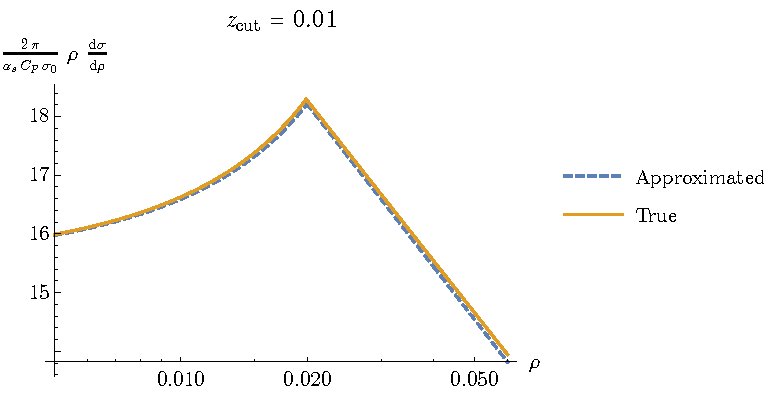
\includegraphics[width=0.9\textwidth]{\main/leading_order/figures/approximation_small_zcut_0.01.pdf}
		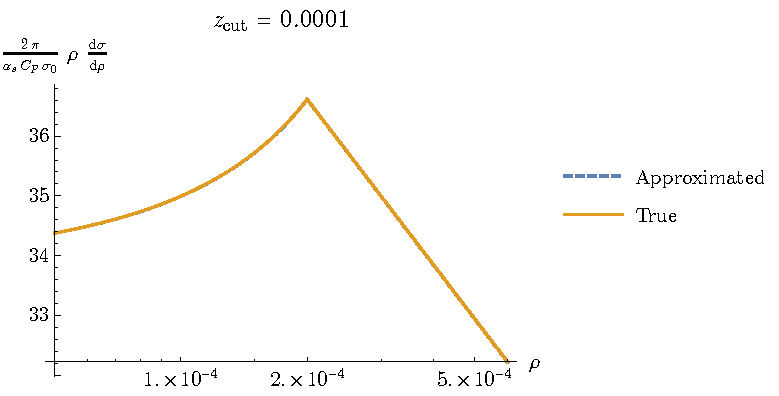
\includegraphics[width=0.9\textwidth]{\main/leading_order/figures/approximation_small_zcut_0.0001.pdf}

		\caption{\label{fig:fixed order approx}True (orange solid line) and approximated (blue dashed line) distribution of groomed heavy hemisphere mass in the limit $\rho \sim \zcut \ll 1$.}
	\end{center}
	\end{figure}

	For this calculation, the true analytic distribution is known completely and can be used for comparison. From Ref.~\cite{larkoski_improving_2020}, we have
	\begin{equation}
	\begin{aligned}
		\frac{2\pi}{\alpha_s C_F}\frac{1}{\sigma_0}\frac{d\sigma}{d\rho} &= \Theta\qty(\frac{3}{4}-\rho)\Theta(\rho - (2\zcut - \zcut^2))\Bigg[ -\frac{12(6-6\sqrt{1-\rho} + \rho(-8 + 5\sqrt{1- \rho} + 2\rho))}{\rho^3(1 - \rho)} \\
		&\qquad- \frac{2(6 - 6 \sqrt{1 - \rho} - \rho(5 - 4\sqrt{1 - \rho}))}{\rho^2(1 - \rho)} \log(\frac{\rho}{2 + 2\sqrt{1 - \rho} - 3\rho}) \Bigg] \\
		&+ \Theta(2\zcut - \zcut^2 - \rho)\Bigg[ \frac{12(1 - 2\zcut)(2 - 2\sqrt{1 - \rho} - \rho)^2}{\rho^3(2 - 2\sqrt{1 - \rho} - \rho(2 - \sqrt{1 - \rho}))} \\ 
		&\hspace{-2cm}- \frac{2(6 -6 \sqrt{1 - \rho} - \rho(5 - 4\sqrt{1 - \rho}))}{\rho^2(1 - \rho)}\log(\frac{2 - 4\zcut(1 - \zcut - \sqrt{1 - \rho}) - 2\sqrt{1 - \rho} - \rho}{4\zcut(1 - \zcut) - \rho})\Bigg].
	\end{aligned}
	\end{equation}
	The true result is plotted against the approximation in Fig.~\ref{fig:fixed order approx}. Notice that, as expected, the approximation gets better both as $\zcut$ becomes smaller and as $\rho$ moves closer to $\zcut$.

	Now, from the true result, we can then take the limit $\rho \sim \zcut \ll 1$ explicitly to find
	\begin{equation}
	\begin{aligned}
		\frac{2\pi}{\alpha_s C_F}\frac{1}{\sigma_0}\frac{d\sigma}{d\rho} &=\Theta(\rho - 2\zcut)\qty[-\frac{3}{\rho} + \frac{4}{\rho} \log(\frac{4}{\rho})] \\
			&\hspace{3cm}+ \Theta(2\zcut - \rho)\qty[ -\frac{3}{\rho} - \frac{4}{\rho}\log(\zcut - \frac{\rho}{4})] \\
		&= \Theta(\rho - 2\zcut)\frac{4}{\rho} \log(\frac{4}{\rho}) \\
			&\hspace{3cm}- \Theta(2\zcut - \rho)\frac{4}{\rho}\log(\zcut - \frac{\rho}{4}) - \frac{3}{\rho}.
	\end{aligned}
	\end{equation}
	Notice as well that taking the same limit in Eq.~\ref{eq:fixed order result} yields
	\begin{equation}
		\frac{2\pi}{\alpha_s C_F}\frac{\rho}{\sigma_0}\frac{d\sigma}{d\rho} = 4\Theta(\rho - 2\zcut)\log(\frac{4}{\rho}) - 4\Theta(2\zcut - \rho)\log(\zcut - \frac{\rho}{4}) - 3,
	\end{equation}
	which is the same result!
	
	Thus, we see that this method works. To compute the distribution in a given limit, it suffices for us to consider only `interesting' regions of phase space, compute their contribution to the distribution, and then combine these contributions in the appropriate manner. The same principle will be applied as we work towards an all-orders calculation. 

	There, too, we will begin by identifying the singular regions of phase space and the dominant physical contributions in each region. We will need to resum the contributions in each region in order to manage the effects of imposed scales to all orders, but this is simply an additional step in the calculation. Moreover, instead of a simple sum, we will combine functions by convolving them, since we need to appropriately capture terms at every order in $\alpha_s$ hidden in each function. Despite these complications, however, the core idea is the same, and this simple example provides a general road map as we push forward.\footnote{We could think of this as a map which only contains the location of the interstate highways.}


\ifstandalone
\bibliographystyle{../bsts/JHEP} 
\bibliography{../jet_substructure}
\fi
\end{document}



\chapter{Factorization formula}

	% This is the Reed College LaTeX thesis template. Most of the work 
% for the document class was done by Sam Noble (SN), as well as this
% template. Later comments etc. by Ben Salzberg (BTS). Additional
% restructuring and APA support by Jess Youngberg (JY).
% Your comments and suggestions are more than welcome; please email
% them to cus@reed.edu
%
% See http://web.reed.edu/cis/help/latex.html for help. There are a 
% great bunch of help pages there, with notes on
% getting started, bibtex, etc. Go there and read it if you're not
% already familiar with LaTeX.
%
% Any line that starts with a percent symbol is a comment. 
% They won't show up in the document, and are useful for notes 
% to yourself and explaining commands. 
% Commenting also removes a line from the document; 
% very handy for troubleshooting problems. -BTS

% As far as I know, this follows the requirements laid out in 
% the 2002-2003 Senior Handbook. Ask a librarian to check the 
% document before binding. -SN

%%
%% Preamble
%%
% \documentclass{<something>} must begin each LaTeX document
% \providecommand{\main}{..}
\documentclass[../thesis.tex]{subfiles}
% \graphicspath{{\subfix{figures/}}}
% Packages are extensions to the basic LaTeX functions. Whatever you
% want to typeset, there is probably a package out there for it.
% Chemistry (chemtex), screenplays, you name it.
% Check out CTAN to see: http://www.ctan.org/
%%
% \usepackage{graphicx,latexsym} 
% \usepackage{amssymb,amsthm,amsmath}
% \usepackage{longtable,booktabs,setspace} 
% \usepackage{chemarr} %% Useful for one reaction arrow, useless if you're not a chem major
% \usepackage[hyphens]{url}
% \usepackage{rotating}
% \usepackage{hyperref}

% \usepackage{physics}
% \usepackage{siunitx}
% \usepackage{xcolor}
% \usepackage{standalone}
% \usepackage{natbib}
% Comment out the natbib line above and uncomment the following two lines to use the new 
% biblatex-chicago style, for Chicago A. Also make some changes at the end where the 
% bibliography is included. 
%\usepackage{biblatex-chicago}
%\bibliography{thesis}

% \usepackage{times} % other fonts are available like times, bookman, charter, palatino

\providecommand{\zcut}{\mathrm{z_{cut}}}


\setlength{\parskip}{0pt}
%%
%% End Preamble
%%
%% The fun begins:
\begin{document}
	Fixed-order calculations like that of Chapter \ref{chap:leading order} are nice because of their exactness, but because of the relatively large value the strong coupling, $\alpha_s \sim 0.1$, one must go to fairly high orders to obtain precision results. At low orders, the calculations are relatively straightforward, but this quickly ceases to be the case, as the number of event topologies that one must consider increases factorially with the order of $\alpha_s$. Moreover, and more pressingly, when we compute an exclusive cross section like $\sigma(e^+ e^- \to \text{hemisphere jets})$ in the presence of mMDT grooming, external energy scales are imposed. This is problematic for QCD, which is an intrinsically scale-invariant theory, and our punishment is the appearance of logarithms of scales which might grow large in particular limits, like the limit $\rho \sim \zcut \ll 1$ which we are considering \cite{larkoski_elementary_2019-1}. All this is to say that, while fixed-order calculations are nice for developing intuition for a physical quantity, they have limitations which become quite severe in the regime in which we are interested.

	We would therefore like to develop an alternative framework for calculating the distribution of heavy hemisphere mass. The strategy we will settle on is try to develop an \textbf{all-orders calculation} of the distribution. This result will take into account contributions at every order of $\alpha_s$, and provide a mathematical structure for producing arbitrarily accurate predictions, given sufficiently precise inputs. We will get there via the process of \textbf{resummation}, which will be discussed in Sec.~\ref{all-sec:resummation} (and, indeed, will occupy most of Chapter \ref{chap:all orders}). In order to prepare for that, we must first lay some groundwork.

	The first step on the path to an all-orders calculation is to derive a factorization formula for the heavy hemisphere mass cross section, the goal being to split the cross section into terms which each depend only on a single energy scale. The basic process for doing so is laid out in technical detail in Ref.~\cite{becher_introduction_2015-1}, and an example of a similar flavor to our calculation is provided by Frye et al.\ in Ref.~\cite{frye_factorization_2016}.\footnote{Indeed, the calculation of Frye et al.\ is a more general factorization of mass-like variables in groomed jets. Setting $\alpha = 2, \beta = 0$ for their two-point energy correlation function $e_2^{(\alpha)}$ under soft drop grooming with angular exponent $\beta$ yields the mMDT-groomed jet mass $\rho$. Their factorization is valid in the limit $\rho \ll \zcut \ll 1$, whereas we are interested in the limit $\rho \sim \zcut \ll 1$.} Once the cross section has been split into functions of single energy scales, the process of resummation can begin. 

	There are two primary steps in developing a factorization formula:
	\begin{enumerate}
		\item \textbf{Power counting}: this involves determining the possible radiative modes of an event and their dominant momentum scales. The term `power counting' refers to the fact that for some momentum scale $\lambda$, different radiative modes have momenta that scale as different powers of $\lambda$.

		\item \textbf{Factorization and refactorization}: Once the different radiative modes and energy scales are identified, we can use the framework of SCET to split the cross section into a convolution of terms describing different radiative modes. These terms themselves must then be split (refactored) into convolutions of terms, each of which depends, to leading order, only on a single energy scale.
	\end{enumerate}
	In this chapter, we will follow these steps to derive a factorization formula for the heavy hemisphere mass in the $\rho \sim \zcut \ll 1$ limit.

\section{Setup}
	Recall that the hemisphere mass is defined to be
	\begin{equation}
		\rho = \frac{1}{E_J^2} \sum_{i<j} 2p_i \cdot p_j
	\end{equation}
	with $E_J$ the jet energy and the sum ranging over all pairs of particles in the jet. Expanding out the dot product, we have
	\begin{equation}\label{factor-eq:jet mass z theta}
		\rho = \frac{2}{E_J^2} \sum_{i<j} \qty(E_i E_j - \vb{p}_i \cdot \vb{p}_j) = \frac{2}{E_J^2} \sum_{i<j} E_i E_j \qty(1 - \cos\theta_{ij}) = \sum_{i<j}2z_i z_j \qty(1 - \cos\theta_{ij}).
	\end{equation}
	Here, $z_i$ and $z_j$ are the relative energy fractions of each particle and $\theta_{ij}$ is the angle between particles $i$ and $j$.

	Throughout the following discussion, with $n^\mu$ the jet direction and $\bar n^\mu$ the direction opposite the jet, we will describe momenta in light-cone coordinates
	\begin{equation}
		p^\mu = \qty(p^-, p^+, p_\perp)
	\end{equation}
	with
	\begin{align}
		p^- &= \bar n \cdot p & p^+ &= n \cdot p
	\end{align}
	and $p_\perp$ the components of momentum transverse to $n$. In these coordinates, the energy fraction with respect to total energy $E_J = Q$ is
	\begin{equation}\label{factor-eq:z light cone coordinates}
		z = \frac{p^+ + p^-}{2Q}
	\end{equation}
	and, in the collinear limit, the angle to the jet axis is $\theta \approx p_\perp / p^0$ \cite{frye_factorization_2016}.
	
	In an $e^+ e^- \to \text{jets}$ event, there are two types of emission: resolved and unresolved. The essential difference is that a resolved emission is one which manifests itself as a jet at a particular scale of observation, while an unresolved emission does not. The presence of unresolved emissions can, however, perturb observable values of a resolved emission. {\color{red}\textbf{[TODO: check that this is a reasonable description]}} 

	Suppose now that we have applied an mMDT groomer with energy fraction cutoff $\zcut$. Then every \textit{resolved} emission must satisfy
	\begin{equation}
		z_i > \zcut,
	\end{equation}
	while other emissions with $z_i < \zcut$ can only pass the groomer if they are at a sufficiently small angle to a resolved emission.

\section{Power counting}
\subsection{Resolved soft emission}
	The primary emission contributing to the jet mass in the limit $\rho \sim \zcut \ll 1$ is a gluon emission $z_i$ sensitive to both $\rho$ and $\zcut$. In the presence of a hard quark (i.e., the jet) with $z_q \sim 1$, leading contributions to the jet mass of Eq.~\ref{factor-eq:jet mass z theta} is
	\begin{equation}
		\rho \approx \sum_i 2z_i \qty(1 - \cos\theta_i)
	\end{equation}
	where $\theta_i$ is the angle of emission $i$ from the quark. Considering the case with only one such emission,\footnote{This is the one-loop contribution {\color{red}\textbf{[is this accurate?]}}.} we have
	\begin{equation}
		\rho \approx z_i \qty(1 - \cos\theta_i).
	\end{equation} 
	But since $z_i \sim \zcut$ and $\rho \sim \zcut$, this means that
	\begin{equation}
		\rho \approx \rho \qty(1 - \cos\theta_i),
	\end{equation}
	so
	\begin{equation}
		\cos\theta_i \ll 1.
	\end{equation}
	This means that
	\begin{equation}
		\theta_i \sim \frac{\pi}{2}.
	\end{equation}
	Since this emission is sensitive to $\zcut \ll 1$, we can also conclude that $z_i \ll 1$. Thus, we see that the leading contribution to the cusp region comes from a \textbf{resolved soft, wide-angle} gluon. Its momentum scales like
	\begin{equation}
		p_R \sim \zcut Q \qty(1, 1, 1).
	\end{equation}
	For future reference, let this gluon have energy fraction $z_R$ and angle $\theta_R$ from the quark axis.

\subsection{Ungroomed extra-soft unresolved radiation}
	\begin{figure}
	\begin{centering}
		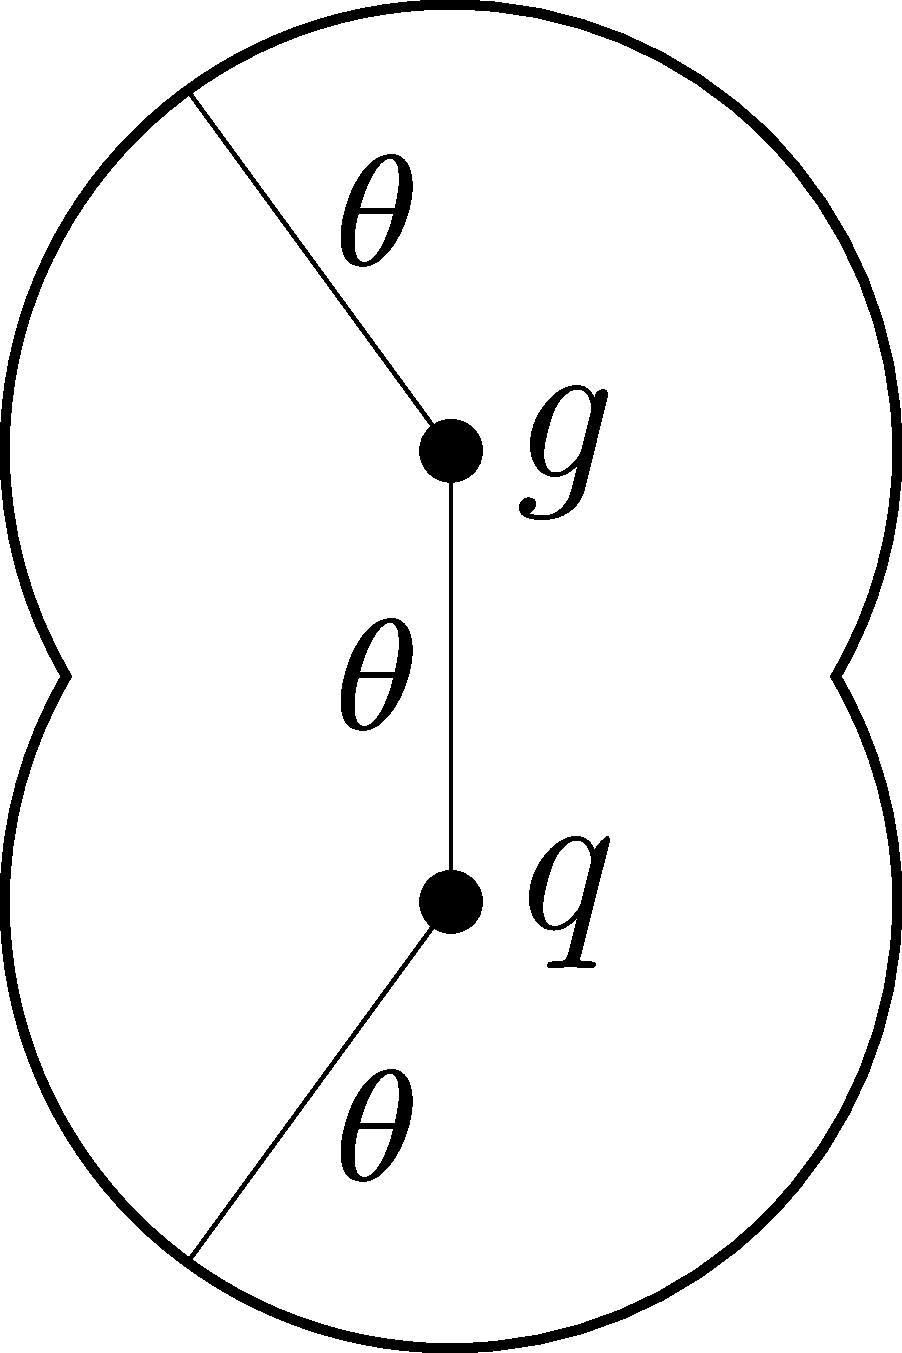
\includegraphics[width=0.2\columnwidth]{figures/head_on_schematic.pdf}
		\caption{\label{fig:head-on schematic}Head-on schematic of a quark jet $q$ and a resolved gluon $g$. If the angle between the quark and the gluon is $\theta$ and the gluon (plus all lower-scale unresolved radiation) passes the groomer, then the mMDT groomer will accept all radiation within an angle $\theta$ of both the quark and the resolved gluon.}
	\end{centering}
	\end{figure}
	Unresolved soft emissions can also contribute to the jet mass if they are sufficiently close to the resolved emission or the quark. Suppose there is another emission $i$ with energy fraction $z_i$ at angle $\theta_i$ from the jet axis and angle $\theta_{iR}$ from the resolved gluon. If $\theta_i < \theta_R$ or $\theta_iR < \theta_R$, a situation displayed in Fig.~\ref{fig:head-on schematic}, then emission $i$ will pass the groomer.

	What does this mean for the hemisphere mass? Well, first notice that since $\theta_R \sim \pi/2$, most soft radiation in the hemisphere passes this cut. The effect of these extra-soft emissions, which have $z_i \ll z_R$, is to perturb the mass of the resolved emission, so that the hemisphere mass is approximately
	\begin{equation}
		\rho \sim z_R + \sum_i z_i(1 - \cos\theta_i).
	\end{equation}
	The dominant contributions come again from the wide-angle emissions with $1 - \cos\theta_i \sim 1$; these must evidently have an energy scale set by
	\begin{equation}
		\rho - z_R \sim \sum_i z_i.
	\end{equation}
	Hence, since $z_R \sim \zcut$, the unresolved extra-soft emissions must scale as
	\begin{equation}
		p_{S_R} \sim \qty(\rho - \zcut)Q(1, 1, 1).
	\end{equation}

% \subsection{Groomed soft radiation}
% 	Radiation outside of the region displayed in Fig.~\ref{fig:head-on schematic} gets groomed away if its energy fraction is
% 	\begin{equation}
% 		z_i < \zcut.
% 	\end{equation}
% 	If $z_i > \zcut$, then we would have a second resolved emission, which we have already decided to ignore. These emissions must be at a very wide angle in order to not be within the region of mMDT acceptance. Since this \textbf{global soft} radiation is removed by the groomer, it is not sensitive to $\rho$ and contributes only to the normalization. It must scale as
% 	\begin{equation}
% 		p_{S_G} \sim \zcut Q(1, 1, 1).
% 	\end{equation}

\subsection{Collinear radiation}\label{sec:collinear radiation}
	Finally, we consider radiation collinear to a jet axis with angle $\theta_i \ll 1$. This radiation has $p^- \gg p^+$, which means from Eq.~\ref{factor-eq:z light cone coordinates} that
	\begin{equation}
		z \approx \frac{p^+}{2Q}.
	\end{equation}
	Then because the particle must satisfy
	\begin{equation}
		z_i \theta_i^2 \lesssim \rho,
	\end{equation}
	we find that \cite{frye_factorization_2016}
	\begin{equation}
		\rho \sim \frac{p^+}{Q}.
	\end{equation}

	If $z \sim 1$, we know that $z \gg \zcut$, so the momentum scales independently of $\zcut$. Hence, the scaling of these \textbf{collinear} modes is \cite{frye_factorization_2016}
	\begin{equation}
		p_c \sim Q \qty(1, \rho, \rho^{1/2}).
	\end{equation}
	In a hemisphere where the resolved emission stops the mMDT groomer, this is the only collinear radiation that contributes {\color{red}\textbf{[TODO: ask Andrew: is this correct?]}}.

	If on the other hand $z \sim \zcut \ll 1$, the result is \textbf{collinear-soft} radiation with $p^- \sim z_i Q$ and $p^+ \sim \theta_i^2 z_i Q$. From \cite{frye_factorization_2016}, these momenta scale like
	\begin{equation}
		p_{cs} \sim \zcut Q \qty(1, \frac{\rho}{\zcut}, \qty(\frac{\rho}{\zcut})^{1/2})
	\end{equation}
	and depend on the single energy scale $\sqrt{\rho\,\zcut}$. This scale matters in the hemisphere which does not contain the resolved soft gluon.


\section{Factorization}
	With the power counting in hand, we are now ready to derive a factorization formula describing the hemisphere mass distribution in the limit $\rho \sim \zcut \ll 1$. First, we should note that it is most straightforward to compute the double differential cross section in the masses of the individual hemispheres, then integrate over them to get the heavy hemisphere mass \cite{chien_resummation_2010}:
	\begin{equation}\label{factor-eq:heavy hemisphere cross section}
		\frac{d\sigma}{d\rho} = \int \frac{d^2\sigma}{d\rho_1d\rho_2}\qty[\delta(\rho - \rho_1)\Theta(\rho_1 - \rho_2) + \delta(\rho - \rho_2)\Theta(\rho_2 - \rho_1)].
	\end{equation}
	The integral simply breaks up the two cases $\rho_1 > \rho_2$ and $\rho_2 > \rho_1$ and assigns the correct value of $\rho$ in each case.

	Now, in the limit $\rho_1, \rho_2 \ll 1$, we can apply the technology of SCET to factorize the double-differential cross section into a product of hard, soft, and jet contributions \cite{frye_factorization_2016,ellis_jet_2010}. The basic form is
	\begin{equation}
		\frac{d^2\sigma}{d\rho_1 d\rho_2} = H(Q^2) \otimes S(\rho_1, \rho_2, \zcut) \otimes J_q(\rho_1) \otimes J_g(\rho_1, \zcut) \otimes J_{\bar q}(\rho_2).
	\end{equation}
	The symbol $\otimes$ represents convolution. Here, $Q^2$ is the squared center-of-mass energy of the collision. $H(Q^2)$ is hard function representing the cross section of $e^+ e^- \to q\bar{q}$ events, $S(\rho_1, \rho_2, \zcut)$ is the function representing soft contributions (which are sensitive to $\zcut$), and $J_i(\rho)$ is a function describing the production of a jet off of particle $i$ (where $i$ is a quark $q$, antiquark $\bar q$, or gluon $g$).

	As this factorization currently stands, several terms depend on multiple scales and must be refactorized. In the limit $\rho \sim \zcut \ll 1$ after mMDT grooming, the soft function consists of global soft emissions which contribute only to the normalization; a resolved soft, wide-angle emission generated by a fixed-order function; and soft radiation which passes the groomer due to the resolved emission. The first two depend only on the scale $\zcut$ and can be combined into one function. Therefore, we can write
	\begin{equation}
	\begin{aligned}
		\frac{d^2\sigma}{d\rho_1 d\rho_2} = H(Q^2) \times R(\rho_1, \rho_2, \zcut) \times S_R(\rho - \zcut) &\otimes J_{c, q}(\rho_1, \zcut)\\
			& \otimes J_{c, g}(\rho_1, \zcut) \otimes J_{c, \bar q}(\rho_2, \zcut).
	\end{aligned}
	\end{equation}
	Here, $R(\rho_1, \rho_2, \zcut)$ describes the resolved emission as well as other soft wide-angle radiation (from which the resolved emission emerged), while $S_R(\rho - \zcut)$ describes radiation which passes the groomer in the presence of the resolved emission. We have also re-written the jet functions as $J_{c, i}(\rho, \zcut)$ to make explicit their dependence on multiple scales.

	Now, as we established in Sec.~\ref{sec:collinear radiation}, radiation collinear to the jet with energy fraction of order 1 depends only on $\rho$, and radiation with energy fraction much less than 1 depends on the scale $\sqrt{\rho\,\zcut}$. However, this soft-collinear radiation only matters in the absence of a resolved gluon emission (which stops the mMDT groomer), in which case the jet function factorizes as
	\begin{equation}
		J_{c, \bar q}(\rho, \zcut) = J_{\bar q}(\rho) \otimes S_C(\sqrt{\rho\,\zcut})
	\end{equation}
	The result is that we must treat each hemisphere separately, since one contains the resolved emission and the other does not. Moreover, the gluon's jet function $J_g$ only depends on the scale of the gluon's energy, which is a function of $\rho$ and $\zcut$ {\color{red}\textbf{[TODO: check this]}}. Therefore, if we assume, without loss of generality, that $\rho_1 > \rho_2$, the cross section becomes
	\begin{equation}\label{factor-eq:factorization formula}
	\boxed{
	\begin{aligned}
		\frac{d^2\sigma}{d\rho_1 d\rho_2} = 2 H(Q^2) \times R(\rho_1, \rho_2, \zcut) &\times S_R(\rho - \zcut) \otimes J_{c, q}(\rho_1)\\
			& \otimes J_{c, g}(\rho_1, \zcut) \otimes \qty[J_{\bar q}(\rho_2) \otimes S_C(\sqrt{\rho_2\,\zcut})].
	\end{aligned}
	}
	\end{equation}
	This is our final factorization formula for the double differential cross section in each hemisphere mass. The distribution of the heavy hemisphere mass then given by Eq.~\ref{factor-eq:heavy hemisphere cross section}. We are now ready to proceed with resummation.

% \ifstandalone
% \bibliographystyle{../bsts/JHEP} 
% \bibliography{../jet_substructure}
% \fi
\end{document}



\chapter{All-orders calculation}
	
	\documentclass[../thesis.tex]{subfiles}

\providecommand{\zcut}{z_\mathrm{{cut}}}
\providecommand{\LIPS}{\mathrm{LIPS}}
\providecommand{\cusp}{\mathrm{cusp}}
\providecommand{\mMDT}{\mathrm{mMDT}}
\providecommand{\Li}{\mathrm{Li}}

\providecommand{\arctanh}{\mathrm{arctanh}}

\providecommand{\cM}{\mathcal{M}}
\providecommand{\cL}{\mathcal{L}}
\providecommand{\cO}{\mathcal{O}}


\setlength{\parskip}{0pt}
%%
%% End Preamble
%%
%% The fun begins:
\begin{document}
	Recall that the goal of our all-orders calculation is to derive an expression which systematically accounts for logarithmic contributions at every order in $\alpha_s$ and with which, if one has sufficient patience and mathematical skill, one could compute the heavy hemisphere mass to arbitrary accuracy in the $\rho \sim \zcut \ll 1$ limit. In this chapter, we will see how this is done.

	As we have repeated several times by now,\footnote{Because it bears repeating!} QCD is a scale-invariant theory. However, when we compute something like the groomed heavy hemisphere mass distribution, we impose scale onto the system (such as the hemisphere mass or the groomer energy cut). In QCD, whenever multiple scales appear, say $\Lambda_h$ and $\Lambda_\ell$, high-order corrections to observables appear with the form \cite{becher_introduction_2015-1}
	\begin{equation}
		\alpha_s^n \log^{n}\frac{\Lambda_h}{\Lambda_\ell}.
	\end{equation}
	These logarithms can grow quite large if the scales are far apart, which enhances the size of these contributions \cite{schwartz_quantum_2014}. Moreover, since these contributions occur at every order in $\alpha_s$, they can be difficult to take care of. This leaves us in a quandary --- how do we handle large corrections which are, for all intents an purposes, out of computational reach?

	The key to an all-orders calculation of the distribution is to keep track of these logarithmic corrections in a systematic way, move them around, and put them back together into a scale-invariant function. This is the process of \textbf{resummation}, which we are about to undertake.

\section{Resummation}\label{all-sec:resummation}
	The first step towards resummation in SCET is to derive a factorization formula \cite{becher_introduction_2015-1}, as we have already done in Eq.~\ref{factor-eq:factorization formula}. Splitting the cross section into terms, each of which depends only on a single scale, enables resummation of each term \cite{frye_factorization_2016}.

	It will be helpful to work in Laplace space, which for a function $f(t)$ is achieved by the transformation \cite{boas_mathematical_2006}
	\begin{equation}
		\cL\qty{f}(s) = \int_0^\infty f(t) e^{-st}\,dt.
	\end{equation}
	For notational simplicity, instead of writing $\cL\qty{f}(s)$ everywhere, we will simply write $f(s)$. That is, whenever a function is written in terms of Laplace variables, we will assume that it is the Laplace-transformed function, and vice versa.

	Under Laplace transformation, convolution becomes multiplication, so under the transformation $\rho \to \nu$, the factorization formula becomes
	\begin{equation}\label{all-eq:factorization formula laplace}
	\begin{aligned}
		\frac{d^2\sigma}{d\nu_1 d\nu_2} = 2 H(Q^2) \times R(\nu_1, \nu_2, \zcut) \times S_R(\nu_1 - \zcut) &\times J_q(\nu_1) \times J_g(\nu_1, \zcut) \\
		&\qquad\times J_{\bar q}(\nu_2) \times S_C(\sqrt{\nu_2 \zcut}).
	\end{aligned}
	\end{equation}
	The multiplicative factorization in Laplace space allows us to resum each term individually, without worrying about cross-talk between terms \cite{frye_factorization_2016}. Before moving on, with this calculation, let us study how our resummation strategy will work.

\subsection{Strategy}
	Let us consider the simple example of a cross section which factorizes into the product of two terms:
	\begin{equation}
		\sigma = F_1 F_2.
	\end{equation}
	Suppose we are working in $d = 4 - 2\epsilon$ dimensions and have introduced a mass scale $\mu$ to compensate for dimensionality changes. We call $\mu$ the \textbf{renormalization scale}. Since $\mu$ is an arbitrary scale introduced to regulate the calculation, the physical quantity $\sigma$ must be independent of $\mu$ at the end of the day:
	\begin{equation}\label{all-eq:partial sigma mu zero}
		\frac{\partial \sigma}{\partial \mu} = 0.
	\end{equation}
	In 4 dimensions, this would be true of $F_1$ and $F_2$ as well. But in our dimensional regularization scheme, away from 4 dimensions, these functions \textit{do} have $\mu$-dependence. Their departure from $\mu$-independence is described by a quantity called the \textbf{anomalous dimension}, so-called because the behavior away from 4 dimensions is anomalous in this sense. If $F_1$ has an anomalous dimension $\gamma_1$ and $F_2$ has an anomalous dimension $\gamma_2$, then it is a general fact of quantum field theory that \cite{schwartz_quantum_2014}
	\begin{align}\label{all-eq:toy RGE}
		\frac{\partial F_1}{\partial \log \mu} &= \gamma_1 F_1 & \frac{\partial F_2}{\partial \log \mu} &= \gamma_2 F_2.
	\end{align}
	In fact, many authors (such as the author of Ref.~\cite{schwartz_quantum_2014}) \textit{define} the anomalous dimension this way. Now notice that this yields, by the product rule,
	\begin{equation}
		\frac{\partial \sigma}{\partial \log \mu} = (\gamma_1 + \gamma_2) F_1 F_2.
	\end{equation}
	In order to enforce Eq.~\ref{all-eq:partial sigma mu zero}, we demand that
	\begin{equation}\label{all-eq:toy anomalous dimension sum}
		\gamma_1 + \gamma_2 = 0.
	\end{equation}
	This provides constraints on our calculations as well as a strong consistency check --- if we have calculated $F_1$ and $F_2$ and find that Eq.~\ref{all-eq:toy anomalous dimension sum} is unsatisfied, then we know a mistake has been made. On the other hand, it means that if we compute the anomalous dimension of $F_1$, then we do not need to compute the anomalous dimension of $F_2$.

	Equations \ref{all-eq:partial sigma mu zero} and \ref{all-eq:toy RGE} are known as \textbf{renormalization group equations}.\footnote{The renormalization group refers to the symmetry of physical quantities under changes in the techniques used to calculate them. Technically, we are working with the \textbf{continuum renormalization group}, which formalizes the independence of observable quantities on $\mu$ in dimensional regularization \cite{schwartz_quantum_2014}.} The overall strategy to resum large logarithms in the cross section $\sigma$ is to solve the renormalization group equation for each function $F_1$ and $F_2$. As long as $\sigma$ factorizes as claimed and Eq.~\ref{all-eq:toy anomalous dimension sum} is satisfied, then this results in an all-orders calculation of $\sigma$.

	Thus, we have a general two-step strategy for resumming a function $F$ (such as $F_1$ or $F_2$ in the example above):
	\begin{enumerate}
		\item Compute the anomalous dimension $\gamma$ of $F$. This is done by computing $F$ to some desired order in $\alpha_s$ and pulling out the appropriate terms. 

		\item Solve the renormalization group equation
		\begin{equation}\label{all-eq:general RGE}
			\frac{\partial F}{\partial \log \mu} = \gamma F = \qty(\Gamma_F(\alpha_s) \log\frac{\mu^2}{\mu_1^2} + \gamma_F(\alpha_s))F.
		\end{equation}
	\end{enumerate}
	These steps are explained in more detail below.

\subsection{Anomalous dimension}

	In order to solve the renormalization group equation, we need to know more about the anomalous dimensions. In general, for a function $F$, the anomalous dimension $\gamma$ can be written as \cite{frye_factorization_2016}
	\begin{equation}\label{all-eq:general anomalous dimension}
		\gamma = \Gamma_F(\alpha_s) \log\frac{\mu^2}{\mu_1^2} + \gamma_F(\alpha_s).
	\end{equation}
	Here, $\mu_1$ is the remainder of the scale appearing with $\mu$ in the logarithm. We call $\Gamma_F(\alpha_s)$ the \textbf{cusp anomalous dimension}, and $\gamma_F(\alpha_s)$ is the \textbf{non-cusp anomalous dimension}. The cusp anomalous dimension is universal up to normalization and can be written as a series in $\alpha_s$:
	\begin{equation}\label{all-eq:general cusp anomalous dimension}
		\Gamma_F(\alpha_s) = d_F \Gamma_\cusp(\alpha_s) = d_F \sum_{n = 0}^\infty \Gamma_n \qty(\frac{\alpha_s}{4\pi})^{n + 1}.
	\end{equation}
	The coefficients $\Gamma_n$ can be pulled from the literature. The relevant terms for our purposes are \cite{frye_factorization_2016}
	\begin{equation}\label{all-eq:Gamma values}
	\begin{aligned}
		\Gamma_0 &= 4 \\
		\Gamma_1 &= 4C_A \qty(\frac{67}{9} - \frac{\pi^2}{3}) - \frac{80}{9}T_R n_f,
	\end{aligned}
	\end{equation}
	where $C_A = 3$ and $T_R = 1/2$ are color factors from QCD and $n_f$ is the number of quarks with energy less than that being considered.

	The real work comes from computing the non-cusp anomalous dimension
	\begin{equation}\label{all-eq:general non-cusp anomalous dimension}
		\gamma_F(\alpha_s) = \sum_{n = 0}^\infty \gamma_n \qty(\frac{\alpha_s}{4\pi})^{n + 1}.
	\end{equation}
	An example calculation will be performed in Sec.~\ref{all-sec:soft function calculation}. This entails computing the function of interest to the desired accuracy, then peeling off the non-logarithmic contributions to the anomalous dimension. The anomalous dimension can be determined either through inspection, by simply taking the coefficient of $2/\epsilon$ (the factor of $2$ comes from the fact that we are working in $d = 4 - 2\epsilon$ dimensions; if we were working in $4 - \epsilon$ dimensions, then we would seek the coefficient of $1/\epsilon$), or by computing the appropriate derivative per the renormalization group equation.

\subsection{Solving the renormalization group equation}\label{all-sec:solving RGE}
	To solve the renormalization group equation, Eq.~\ref{all-eq:general RGE}, it is convenient to rewrite the differential equation not in terms of $\mu$, but in terms of $\alpha_s$. This is done through the QCD $\beta$-function, which describes how $\alpha_s$ depends on the energy scale $\mu$ \cite{frye_factorization_2016}:
	\begin{equation}\label{all-eq:beta function definition}
		d\log\mu = \frac{d\mu}{\mu} = \frac{d\alpha_s}{\beta(\alpha_s)}.
	\end{equation}
	This is a manifestation of the running of the coupling $\alpha_s$. The $\beta$-function is another quantity well-known in the literature as a series in $\alpha_s$:
	\begin{equation}
		\beta(\alpha_s) = -2\alpha_s \sum_{n = 0}^\infty \beta_n \qty(\frac{\alpha_s}{4\pi})^{n + 1}
	\end{equation}
	with \cite{frye_factorization_2016}
	\begin{equation}
	\begin{aligned}
		\beta_0 &= \frac{11}{3} C_A - \frac{4}{3}T_R n_f \\
		\beta_1 &= \frac{34}{3} C_A^2 - 4 T_R n_f \qty(C_F + \frac{5}{3} C_A),
	\end{aligned}
	\end{equation}
	where $C_F = 4/3$ is another QCD color factor. The general solution to the renormalization group equation is then \cite{frye_factorization_2016}
	\begin{equation}\label{all-eq:RGE general solution}
	\boxed{
	\begin{aligned}
		F(\mu) = F(\mu_0) \exp\Bigg[ 2 \int_{\alpha_s(\mu_0)}^{\alpha_s(\mu)} \frac{d\alpha}{\beta(\alpha)}\Gamma_F(\alpha) \int_{\alpha_s(\mu_0)}^\alpha \frac{d\alpha'}{\beta(\alpha')} &+ \int_{\alpha_s(\mu_0)}^{\alpha_s(\mu)} \frac{d\alpha}{\beta(\alpha)}\gamma_F(\alpha) \\
		&\hspace{-1cm}+ \log\frac{\mu_0^2}{\mu_1^2} \int_{\alpha_s(\mu_0)}^{\alpha_s(\mu)} \frac{d\alpha}{\beta(\alpha)}\Gamma_F(\alpha) \Bigg].
	\end{aligned}
	}
	\end{equation}
	Here, $\mu_0$ is some reference energy scale of our choosing. One way to think about resummation is that it allows us to compute the function $F$ at any scale $\mu$, given the value at a particular scale $\mu_0$. Moreover, the only place where large logarithms could now live is in $F(\mu_0)$ --- it turns out that the logarithms will contain factors of $\mu_0$, so we can cleverly pick $\mu_0$ in order to eliminate them.

	To see that Eq.~\ref{all-eq:RGE general solution} solves the renormalization group equation \ref{all-eq:general RGE}, we can simply differentiate it with respect to $\mu$. To do so, first notice that
	\begin{equation}
	\begin{aligned}
		\frac{\partial}{\partial \mu} \int_{\alpha_s(\mu_0)}^{\alpha_s(\mu)} \frac{d\alpha}{\beta(\alpha)}\Gamma_F(\alpha) \int_{\alpha_s(\mu_0)}^\alpha \frac{d\alpha'}{\beta(\alpha')} = \frac{\partial \alpha_s(\mu)}{\partial \mu} \frac{\Gamma_F(\alpha_s(\mu))}{\beta(\alpha_s(\mu))} \int_{\alpha_s(\mu_0)}^{\alpha_s(\mu)} \frac{d\alpha}{\beta(\alpha)}.
	\end{aligned}
	\end{equation}
	By the definition of the $\beta$-function in Eq.~\ref{all-eq:beta function definition},
	\begin{equation}
		\frac{\partial \alpha_s(\mu)}{\partial \mu} = \frac{\beta(\alpha_s(\mu))}{\mu}
	\end{equation}
	and
	\begin{equation}
		\int_{\alpha_s(\mu_0)}^{\alpha_s(\mu)} \frac{d\alpha}{\beta(\alpha)} = \int_{\mu_0}^\mu \frac{d\mu'}{\mu'} = \log\frac{\mu}{\mu_0}.
	\end{equation}
	Thus,
	\begin{equation}
		\frac{\partial}{\partial \mu} \int_{\alpha_s(\mu_0)}^{\alpha_s(\mu)} \frac{d\alpha}{\beta(\alpha)}\Gamma_F(\alpha) \int_{\alpha_s(\mu_0)}^\alpha \frac{d\alpha'}{\beta(\alpha')} = \frac{\Gamma_F(\alpha_s(\mu))}{\mu} \log \frac{\mu}{\mu_0}.
	\end{equation}
	The second and third integrals of Eq.~\ref{all-eq:RGE general solution} are similar but more straightforward:
	\begin{align}
		\int_{\alpha_s(\mu_0)}^{\alpha_s(\mu)} \frac{d\alpha}{\beta(\alpha)}\gamma_F(\alpha) &= \frac{\gamma_F(\alpha_s(\mu))}{\mu}, & \int_{\alpha_s(\mu_0)}^{\alpha_s(\mu)} \frac{d\alpha}{\beta(\alpha)}\Gamma_F(\alpha) &= \frac{\Gamma_F(\alpha_s(\mu))}{\mu}.
	\end{align}
	Therefore, differentiating Eq.~\ref{all-eq:RGE general solution} with respect to $\mu$ yields, via the chain rule,
	\begin{equation}
	\begin{aligned}
		\mu \frac{\partial F(\mu)}{\partial \mu} &= F(\mu) \qty[\log\frac{\mu^2}{\mu_0^2} \Gamma_F(\alpha_s) + \gamma_F(\alpha_s) + \log\frac{\mu_0^2}{\mu_1^2}\Gamma_F(\alpha_s)] \\
		&= F(\mu) \qty[\Gamma_F(\alpha_s)\log\frac{\mu^2}{\mu_1^2} + \gamma_F(\alpha_s)],
	\end{aligned}
	\end{equation}
	where we have assigned $\alpha_s = \alpha_s(\mu)$. This is exactly the renormalization group equation, so the solution works.

\subsubsection{Next-to-leading-logarithmic accuracy}\label{all-sec:NLL resummation}
	In a standard perturbative expansion of a physical quantity
	\begin{equation}
		f(\lambda) = \sum_{n = 0}^\infty f_n \lambda^n,
	\end{equation}
	we might talk about approximating a solution by keeping only, say, the leading-order (LO) term $f_0$. If we need higher precision,\footnote{Or are feeling particularly fancy.} we can take higher-order terms in the series, moving to next-to-leading order (NLO), then next-to-next-to-leading-order (NNLO), and so on.

	In the context of a perturbative resummation calculation such as the one at hand, it does not make sense to discuss the order of a result. This is because the exponent of the solution to the renormalization group equation, Eq.~\ref{all-eq:RGE general solution}, is itself a series in $\alpha_s$. To achieve a more accurate result, we want to expand the \textit{exponent} to a fixed order, which means that the quantity itself is \textit{logarithmically} accurate with respect to this expansion. A leading-order exponential expansion yields an overall result accurate to the leading logarithm (LL) of the exponent. Moving to higher accuracy then takes us to the next-to-leading-logarithm (NLL), and so on.

	Whereas LL accuracy gives only the vaguest hints about the distribution of an observable, NLL accuracy is the first order which makes meaningful predictions about the shape of the distribution. For this reason, we will explore the process of developing an NLL calculation.

	To do this, we have to decide how accurately to calculate each piece of Eq.~\ref{all-eq:RGE general solution}. Let
	\begin{equation}
		K(\mu, \mu_0) \equiv 2 \int_{\alpha_s(\mu_0)}^{\alpha_s(\mu)} \frac{d\alpha}{\beta(\alpha)}\Gamma_F(\alpha) \int_{\alpha_s(\mu_0)}^\alpha \frac{d\alpha'}{\beta(\alpha')} + \int_{\alpha_s(\mu_0)}^{\alpha_s(\mu)} \frac{d\alpha}{\beta(\alpha)}\gamma_F(\alpha)
	\end{equation}
	and
	\begin{equation}
		\omega(\mu, \mu_0) \equiv \int_{\alpha_s(\mu_0)}^{\alpha_s(\mu)} \frac{d\alpha}{\beta(\alpha)}\Gamma_F(\alpha).
	\end{equation}
	To achieve NLL accuracy, we want to determine $K(\mu, \mu_0)$ to order $\cO(\alpha_s^0)$, while we want $\omega(\mu, \mu_0)$ to order $\cO(\alpha_s)$ \cite{frye_factorization_2016}. It turns out that we need $\Gamma_\cusp(\alpha_s)$ to order $\cO(\alpha_s^2)$ and $\beta(\alpha_s)$ to order $\cO(\alpha_s^3)$, while we only need the non-cusp anomalous dimension $\gamma_F(\alpha_s)$ to order $\cO(\alpha_s)$. If we take
	\begin{align}
		\Gamma_\cusp(\alpha_s) &= \Gamma_0 \frac{\alpha_s}{4\pi} + \Gamma_1 \qty(\frac{\alpha_s}{4\pi})^2 + \cO(\alpha_s^3) \\
		\gamma_F(\alpha_s) &= \gamma_0 \frac{\alpha_s}{4\pi} + \cO(\alpha_s^2) \\
		\beta(\alpha_s) &= -2\beta_0 \frac{\alpha_s^2}{4\pi} - 2\beta_1 \frac{\alpha_s^3}{(4\pi)^2} + \cO(\alpha_s^4)
	\end{align}
	and let
	\begin{equation}
		r \equiv \frac{\alpha_s(\mu)}{\alpha_s(\mu_0)},
	\end{equation}
	then the first term in the exponent becomes
	\begin{equation}\label{all-eq:NLL K function}
	\begin{aligned}
		K(\mu, \mu_0) = \frac{d_F \Gamma_0}{2\beta_0^2}\Bigg[\frac{4\pi}{\alpha_s(\mu_0)} \qty(\log r + \frac{1}{r} - 1) + \log r \qty(\frac{\beta_1}{\beta_0} - \frac{\Gamma_1}{\Gamma_0}) &+ \frac{\beta_1}{2\beta_0}\log^2 r \Bigg] \\
		&\hspace{-0.75cm}- \frac{\gamma_0}{2\beta_0} \log r + \cO(\alpha_s).
	\end{aligned}
	\end{equation}
	while the second is
	\begin{equation}\label{all-eq:NLL omega function}
		\omega(\mu, \mu_0) = \frac{d_F \Gamma_0}{2\beta_0}\qty[\log \frac{1}{r} + \frac{\alpha_s(\mu_0)}{4\pi}(r - 1)\qty(\frac{\beta_1}{\beta_0} - \frac{\Gamma_1}{\Gamma_0})] + \cO(\alpha_s^2).
	\end{equation}
	Recall that $\Gamma_F(\alpha_s) = d_F \Gamma_\cusp(\alpha_s)$ for some normalization $d_F$.

	With these expansions in place, we can re-write Eq.~\ref{all-eq:RGE general solution} \textit{in Laplace space} as
	\begin{equation}\label{all-eq:NLL RGE solution Laplace}
	\boxed{
		F(\mu) = F(\mu_0) e^{K(\mu, \mu_0)} \qty(\frac{\mu_0^2}{\mu_1^2})^{\omega(\mu, \mu_0)}.
	}
	\end{equation}
	Everything is now defined in terms of known constants and the anomalous dimension except for $F(\mu_0)$. This quantity is determined by calculating $F$ at some fixed order and then evaluating at the scale $\mu_0$.\footnote{$F(\mu_0)$ is simply a boundary value for the renormalization group equation.} {\color{red}\textbf{[TODO: explicate the subtle difference between the resummed result and the fixed-order result. Explain why we needed to go through the trouble of resummation in the first place]}}

\subsection{Full resummed result}\label{all-sec:full resummed result}
	The above process can be completed for every term in the factorization formula, Eq.~\ref{all-eq:factorization formula laplace}. Letting $\mu_F$ be the fixed scale at which function $F$ is evaluated and $\mu_{1, F}$ be the natural scale appearing logarithmically in $F$, we have
	\begin{equation}\label{all-eq:full resummed result Laplace}
	\begin{aligned}
		\frac{d^2\sigma}{d\nu_1 d\nu_2} &= 2 \exp\Bigg[K_H(\mu, \mu_H)  + K_R(\mu, \mu_R) + K_{S_R}(\mu, \mu_{S_R}) + K_{J_q}\qty(\mu, \mu_{J_q})  \\
		&\hspace{4cm}+ K_{J_g}\qty(\mu, \mu_{J_g}) + K_{J_{\bar q}}\qty(\mu, \mu_{J_{\bar q}}) + K_{S_C}(\mu, \mu_{S_C}) \Bigg] \\
		&\hspace{1cm}\times H(Q, \mu_H) R(\nu_1, \nu_2, \zcut, \mu_R) S_R(\nu_1, \zcut, \mu_{S_R}) J_q(\nu_1, \mu_{J_q}) \\
		&\hspace{1cm}\times J_g(\nu_1, \zcut, \mu_{J_g}) J_{\bar q}(\nu_2, \mu_{J_{\bar q}}) S_C(\nu_2, \zcut, \mu_{S_C}) \qty(\frac{\mu_H}{\mu_{1, H}})^{\omega_H(\mu, \mu_H)} \\
		&\hspace{1cm}\times  \qty(\frac{\mu_R}{\mu_{1, R}})^{\omega_R(\mu, \mu_R)} \qty(\frac{\mu_H}{\mu_{1, H}})^{\omega_{S_R}(\mu, \mu_{S_R})} \qty(\frac{\mu_{J_q}}{\mu_{1, J_q}})^{\omega_{J_q}(\mu, \mu_{J_q})} \\
		&\hspace{1cm}\times  \qty(\frac{\mu_{J_g}}{\mu_{1, J_g}})^{\omega_{J_g}\qty(\mu, \mu_{J_g})} \qty(\frac{\mu_{J_{\bar q}}}{\mu_{1, J_{\bar q}}})^{\omega_{J_{\bar q}}\qty(\mu, \mu_{J_{\bar q}})} \qty(\frac{\mu_{S_C}}{\mu_{1, S_C}})^{\omega_{S_C}(\mu, \mu_{S_C})}.
	\end{aligned}
	\end{equation}
	This result is in Laplace space, but we would like it to be in real space. For the function $H$, its lack of $\nu$-dependence means that it does not change under inverse Laplace transformation. However, to transform the rest, we need to be sneaky.

	For any resummed function $F$ appearing in the factorization formula which takes the form (where we have made the $\nu$-dependence in the scale $\mu_1$ explicit)
	\begin{equation}
		F(\nu, \mu) = e^{K(\mu, \mu_0)} F(\nu, \mu_0) \qty(\frac{\nu^\xi \mu_0}{\mu_1})^{\omega(\mu, \mu_0)},
	\end{equation}
	the fixed-scale function $F(\nu, \mu_0)$ contains logarithms of the form \cite{frye_factorization_2016}
	\begin{equation}
		\log^n \frac{\nu^\xi \mu_0}{\mu_1}.
	\end{equation}
	In fact, all $\nu$-dependence will appear in this way.\footnote{If this seems weird now, do not worry. We will see a concrete example later which makes this point clearer. This will be a `proof by example,' if you will.} We can therefore use the clever relationship \cite{becher_factorization_2007,frye_factorization_2016}
	\begin{equation}
		\frac{\partial^n}{\partial q^n} \nu^q = \nu^q \log^n \nu
	\end{equation}
	to re-write the logarithms in the fixed-scale as derivatives. That is, we will take {\color{red}\textbf{[TODO: check this]}}
	\begin{equation}
		\log^n \frac{\nu^\xi \mu_0}{\mu_1} \to \partial^n_{\omega},
	\end{equation}
	a derivative with respect to the function $\omega(\mu, \mu_0)$. Denoting this transformation by $F(L \to \partial_\omega)$, we have
	\begin{equation}
		F(\nu, \mu) = e^{K(\mu, \mu_0)} F(L \to \partial_\omega) \qty(\frac{\nu^\xi \mu_0}{\mu_1})^{\omega(\mu, \mu_0)}.
	\end{equation}
	Now our problem is solved because the inverse Laplace transformation commutes with derivatives and the following transformation is known \cite{frye_factorization_2016}:
	\begin{equation}
		\cL^{-1}\qty{\nu^q} = \frac{\rho^{-q - 1}}{\Gamma(-q)}
	\end{equation}
	where $\rho$ is the transformation partner of $\nu$ and $\Gamma(x)$ is the standard gamma function. Hence, the inverse Laplace transformation of $F(\nu, \mu)$ is
	\begin{equation}\label{all-eq:resummed inverse Laplace transform}
		F(\rho, \mu) = e^{K(\mu, \mu_0)} F(L \to \partial_\omega)\qty[\frac{\mu_0}{\rho^\xi\mu_1}]^{\omega(\mu, \mu_0)} \frac{1}{\rho\,\Gamma(-\xi \omega(\mu, \mu_0))}.
	\end{equation}
	Performing this operation for every term in Eq.~\ref{all-eq:full resummed result Laplace} that has explicit $\nu$-dependence, we have
	\begin{equation}\label{all-eq:full resummed result}
	\boxed{
	\begin{aligned}
		\frac{d^2\sigma}{d\rho_1 d\rho_2} &= 2 \exp\Bigg[K_H(\mu, \mu_H)  + K_R(\mu, \mu_R) + K_{S_R}(\mu, \mu_{S_R}) + K_{J_q}\qty(\mu, \mu_{J_q})  \\
		&\hspace{4cm}+ K_{J_g}\qty(\mu, \mu_{J_g}) + K_{J_{\bar q}}\qty(\mu, \mu_{J_{\bar q}}) + K_{S_C}(\mu, \mu_{S_C})  \Bigg] \\
		&\hspace{1cm}\times H(Q, \mu_H) R(L \to \partial_{\omega_R}) S_R(L \to \partial_{\omega_{S_R}}) J_q(L \to \partial_{\omega_{J_q}}) \\
		&\hspace{1cm}\times J_g(L \to \partial_{\omega_{J_g}}) J_{\bar q}(L \to \partial_{\omega_{J_{\bar q}}}) S_C(L \to \partial_{\omega_{S_C}}) \qty(\frac{\mu_H}{\mu_{1, H}})^{\omega_H(\mu, \mu_H)} \\
		&\hspace{1cm}\times  \qty(\frac{\mu_R}{\mu_{1, R}})^{\omega_R(\mu, \mu_R)} \qty(\frac{\mu_{S_R}}{\mu_{1, {S_R}}})^{\omega_{S_R}(\mu, \mu_{S_R})} \qty(\frac{\mu_{J_q}}{\mu_{1, J_q}})^{\omega_{J_q}\qty(\mu, \mu_{J_q})} \\
		&\hspace{1cm}\times \qty(\frac{\mu_{J_g}}{\mu_{1, J_g}})^{\omega_{J_g}\qty(\mu, \mu_{J_g})} \qty(\frac{\mu_{J_{\bar q}}}{\mu_{1, J_{\bar q}}})^{\omega_{J_{\bar q}}\qty(\mu, \mu_{J_{\bar q}})} \qty(\frac{\mu_{S_C}}{\mu_{1, S_C}})^{\omega_{S_C}(\mu, \mu_{S_C})} \\
		&\hspace{1cm}\times \frac{1}{\rho_1 \rho_2} \frac{1}{\Gamma(-\xi_{J_{\bar q}} \omega_{J_{\bar q}}(\mu, \mu_{J_{\bar q}}) - \xi_{S_C} \omega_{S_C}(\mu, \mu_{S_C}))}   \\
		&\hspace{1cm}\times \frac{1}{\Gamma(-\xi_R \omega_R(\mu, \mu_R) - \xi_{S_R} \omega_{S_R}(\mu, \mu_{S_R}) - \xi_{J_q} \omega_{J_q}(\mu, \mu_{J_q}) - \xi_{J_g} \omega_{J_g}(\mu, \mu_{J_g}))},
	\end{aligned}
	}
	\end{equation}
	where $\xi_F$ is the exponent of $\nu$ in the exponentiated term corresponding to function $F$. The replacement of $\nu \to 1/\rho$ in the exponentiated scale ratios is implicit.
	
	As messy as Eq.~\ref{all-eq:full resummed result} may be, it is remarkable that we can write down the solution in closed form (assuming that we can compute the $K$ and $\omega$ functions). All that is left to do now is compute each piece of the cross section to determine the anomalous dimensions and fixed-scale contributions.

	Luckily for us, several of the functions --- the hard function $H$, the jet functions $J_q$, $J_{\bar q}$, and $J_g$, and the collinear-soft function $S_C$ --- have already been computed to the necessary order for an NLL calculation of the heavy hemisphere mass (see the appendices of Ref.~\cite{frye_factorization_2016}). However, the resolved emission function $R$ and the soft function $S_R$ are novel; for these, we must compute their anomalous dimensions and fixed-scale contributions to order $\alpha_s$. To see how this works, we will compute the soft function $S_R$ in Sec.~\ref{all-sec:soft function calculation}.
	

\section{Soft function}\label{all-sec:soft function calculation}
\subsection{Setup}
	Let us first remind ourselves what it is we are calculating. The soft function $S_R(\rho - \zcut)$ describes soft radiation which passes the mMDT groomer due to its proximity to the resolved gluon. If the resolved emission occurs at an angle $\theta$ from the quark axis, then because of the iterative selection approach of the mMDT grooming algorithm, any radiation at a smaller angle either from the quark or the gluon will pass the groomer.

	We want to compute $S_R$ to order $\alpha_s$, then use the renormalization group equation to resum the soft function. For the sake of this section, let $\rho_s = \rho - \zcut$ be the contribution of the soft ungroomed emissions to the hemisphere mass.

	For now, let the resolved gluon have momentum $k_g$, let the quark lie along the direction $n_q = (1, 0, 0, 1)$, and consider an extra-soft gluon that has been emitted with momentum $k$. If this extra-soft gluon is closer to the quark, then its dominant contribution to the mass $\rho_s$ will come from its interaction with the quark:
	\begin{equation}
		\rho_s = \frac{4k^+}{Q},
	\end{equation}
	where $k^+ = n_q \cdot k$ and $k^- = k \cdot (1, 0, 0, -1)$ are light-cone coordinates with respect to the quark axis. On the other hand, if the extra-soft gluon is closer to the resolved gluon, then its dominant contribution comes from this interaction:
	\begin{equation}
		\rho_s = \frac{4 k \cdot n_g}{Q} = \frac{4 k \cdot k_g}{E_g Q}
	\end{equation}
	where $n_g$ is the direction of the resolved gluon and $k_g$ is its energy.

	Notice now that the angle between the extra-soft gluon and the quark is given by
	\begin{equation}
		1 - \cos\theta_{gq} = \frac{k^+}{k_0},
	\end{equation}
	while the angle between the extra-soft gluon and the resolved gluon is
	\begin{equation}
		1 - \cos\theta_{gg} = \frac{k \cdot n_g}{k_0}.
	\end{equation}
	The case in which the extra-soft gluon is closer to the quark is the case in which $\theta_{gq} < \theta_{gg}$, so $1 - \cos\theta_{gq} < 1 - \cos\theta_{gg}$ and therefore, in turn, $k^+ < k \cdot n_g$. The total measurement function will therefore be
	\begin{equation}
		\delta_{\rho_s} = \Theta\qty(k \cdot n_g - k^+) \delta\qty(\rho - \frac{4 k^+}{Q}) + \Theta\qty(k^+ - k \cdot n_g) \delta\qty(\rho - \frac{4 k \cdot n_g}{Q}).
	\end{equation}

	We also need to impose the kinematic constraint that the extra-soft gluon is sufficiently close to the quark or resolved gluon. Saying that the gluon is in the region is equivalent to saying that it is not outside of the region. The gluon is outside of the quark's radius of influence if
	\begin{equation}
		\frac{k^+}{k_0} = 1 - \cos\theta_{gq} > 1 - \cos\theta = n_g \cdot n_q.
	\end{equation}
	On the other hand, the gluon is outside the resolved gluon's radius of influence if
	\begin{equation}
		\frac{k \cdot n_g}{k_0} = 1- \cos\theta_{gg} > 1 - \cos\theta = n_g \cdot n_q.
	\end{equation}
	Therefore, the mMDT grooming restriction is
	\begin{equation}
		\Theta_\mMDT = 1 - \Theta\qty(k^+ - k_0 \n_g \cdot n_q) \Theta(k\cdot n_g - k_0 n_g \cdot n_q).
	\end{equation}

	In QCD, the gluon carries color charge, so a gluon can be emitted off of any pair of color-charged particles: the quark and antiquark, the quark and resolved gluon, or the antiquark and resolved gluon. The matrix element accounts for all of these possibilities, and in the soft limit in $d = 4 - 2\epsilon$ dimensions it takes the form \cite{catani_infrared_2000}
	\begin{equation}
		\abs{\cM}^2 = -4\pi\alpha_s \mu^{2\epsilon} \sum_{i < j} \vb{T}_i \cdot \vb{T}_j \frac{n_i \cdot n_j}{(n_i \cdot k) (n_j \cdot k)}.
	\end{equation}
	{\color{red}\textbf{[TODO: are we missing a factor of $\sigma_0$?]}} Here $i, j$ range over all the pairs of resolved particles, the $n_i$ are direction vectors, and the $\vb{T}_i$ are color charge matrices which account for color correlations. Their precise definition is unimportant, and all we need to know is that $\vb{T}_q \cdot \vb{T}_{\bar q} = -C_F$ \cite{catani_infrared_2000}.

	For a complete calculation, we would need to compute the soft function separately for each term of the sum, then combine them all together at the end. However, only one of the terms --- emission off of the quark-antiquark pair --- is analytically tractable, so for the sake of demonstration we will focus solely on that. This is equivalent, in some sense, to computing the soft function in a theory like quantum electrodynamics, in which the force carrier does not carry charge.\footnote{Of course, this would be a logically incoherent calculation, as the very presence of jet physics is a result of the particular nonlinearities of QCD which lead to the gluon carrying color charge. Nevertheless, we will continue, since the goal of this thesis is, in large part, pedagogical --- I warned you that we would have to make sacrifices.} Thus, we will simply take
	\begin{equation}
		\abs{\cM}^2 = 4\pi\alpha_s C_F \mu^{2\epsilon} \frac{n_q \cdot n_{\bar q}}{(n_q \cdot k) (n_{\bar q} \cdot k)} = 4\pi\alpha_s C_F \mu^{2\epsilon} \frac{2}{k^+ k^-},
	\end{equation}
	where $n_{\bar q} = (1, 0, 0, -1)$.

	Finally, the phase space measure in $d = 4 - 2\epsilon$ dimensions takes the usual form
	\begin{equation}
		d\Pi = \frac{d^d k}{(2 \pi)^{d - 1}} \delta(k^2) \Theta(k^+) \Theta(k^- - k^+).
	\end{equation}
	{\color{red}\textbf{[TODO: check the power of $2\pi$]}} Notice that we are enforcing the gluon to be emitted in the hemisphere with the quark by requiring $k^- > k^+$. This is necessary because of the assumption we have made in writing the all-orders result of Eq.~\ref{all-eq:full resummed result}. Note as well that we are only scanning over the momentum of the extra-soft gluon: under the assumption that this gluon is softer than the resolved gluon, the emission does not meaningfully influence the momentum of either the quarks or the resolved gluon.

	Thus, putting everything together, we find
	\begin{equation}\label{all-eq:soft function general coords}
	\boxed{
	\begin{aligned}
		S_R(\rho_s) = 4&\pi\alpha_s C_F \mu^{2\epsilon} \int \frac{d^d k}{(2\pi)^{d - 1}} \delta(k^2) \Theta(k^+) \Theta(k^- - k^+) \frac{2}{k^+ k^-} \\
		&\times \qty[\Theta\qty(k \cdot n_g - k^+) \delta\qty(\rho - \frac{4 k^+}{Q}) + \Theta\qty(k^+ - k \cdot n_g) \delta\qty(\rho - \frac{4 k \cdot n_g}{Q})] \\
		&\times \qty[1 - \Theta\qty(k^+ - k_0 \n_g \cdot n_q) \Theta(k\cdot n_g - k_0 n_g \cdot n_q)].
	\end{aligned}
	}
	\end{equation}

\subsection{Coordinate choice}
	If we want to perform any actual calculations, we need to pick a coordinate system in which to evaluate the integral of Eq.~\ref{all-eq:soft function general coords}. Notice that, physically, there is an axial symmetry to the problem: nothing depends on the azimuthal angle of the resolved emission about the quark axis. Therefore, we might define our momenta in terms of the \textbf{detector coordinates} of transverse momentum $p_\perp \in [0, \infty)$, pseudorapidity $\eta \in [0, \infty)$, and azimuthal angle $\phi \in [0, \pi]$. These are defined in terms of Cartesian coordinates $(p_x, p_y, p_z)$ as
	\begin{align}
		p_x &= p_\perp \cos\phi & p_y &= p_\perp \sin\phi & p_z &= p_\perp \sinh\eta \\
		p_\perp &= \sqrt{p_x^2 + p_y^2} & \phi &= \arctan\frac{p_y}{p_x} & \eta &= \arctanh\frac{p_z}{\abs{\vb{p}}}.
	\end{align}
	Notice also that, for an on-shell particle,
	\begin{equation}
		p_0 = \sqrt{p_x^2 + p_y^2 + p_z^2} = p_\perp \cosh\eta.
	\end{equation}
	Define the detector coordinates of the extra soft gluon as $k = (k_0, k_\perp, \phi_k, \eta_k)$.

	The resolved gluon is fixed from the perspective of the extra-soft gluon, so we can write its momentum in whichever coordinates are most convenient. This turns out to be standard spherical coordinates, in which the gluon is emitted with an azimuthal angle $\phi_g$ and a polar angle $\theta_g$ from the jet axis. Without loss of generality, we can define our coordinate axes so that $\phi_g = 0$.

	Now we can transform each term of Eq.~\ref{all-eq:soft function general coords}. First, notice that
	\begin{equation}
		k^+ = k_0 - k_z = k_\perp (\cosh\eta_k - \sinh\eta_k) = k_\perp e^{-\eta_k},
	\end{equation}
	and similarly
	\begin{equation}
		k^- = k_\perp e^{\eta_k}.
	\end{equation}
	Then the restriction $k^+ > 0$ becomes $k_\perp > 0$ and $k^- > k^+$ becomes $\eta_k > 0$. That is,
	\begin{equation}\label{all-eq:phase space constraints specific coords}
		\Theta(k^+) \Theta(k^- - k^+) = \Theta(k_\perp)\Theta(\eta_k).
	\end{equation}
	Moreover, the matrix element becomes
	\begin{equation}\label{all-eq:matrix element specific coords}
		\abs{\cM}^2 = 4\pi\alpha_s C_F \frac{2}{k_\perp^2}.
	\end{equation}

	Next comes the measurement function. Notice that
	\begin{equation}
	\begin{aligned}
		k \cdot n_g &= \qty(k_\perp \cosh\eta_k, k_\perp \cos\phi_k, k_\perp \sin\phi_k, k_\perp \sinh\eta_k) \cdot(1, \sin\theta_g, 0, \cos\theta_g) \\
		&= k_\perp \qty[\cosh\eta_k - \cos\phi_k \sin\theta_g - \sinh\eta_k \cos\theta_g].
	\end{aligned}
	\end{equation}
	Therefore
	\begin{equation}
		\Theta(k^+ - k \cdot n_g) = \Theta\qty(\cos\phi_k \cot\frac{\theta_g}{2} - \sinh\eta_k)
	\end{equation}
	and
	\begin{equation}
		\Theta(k \cdot n_g - k^+) = \Theta\qty(\sinh\eta_k - \cos\phi_k \cot\frac{\theta_g}{2}).
	\end{equation}
	The full measurement function becomes
	\begin{equation}\label{all-eq:measurement function specific coords}
	\begin{aligned}
		\delta_{\rho_s} &= \Theta\qty(\sinh\eta_k - \cos\phi_k \cot\frac{\theta_g}{2}) \delta\qty(\rho_s - \frac{4k_\perp e^{-\eta_k}}{Q}) \\
		&\qquad+ \Theta\qty(\cos\phi_k \cot\frac{\theta_g}{2} - \sinh\eta_k) \delta\qty(\rho_s - \frac{4k_\perp}{Q}\qty[\cosh\eta_k - \cos\phi_k \sin\theta_g - \sinh\eta_k \cos\theta_g]).
	\end{aligned}
	\end{equation}

	We also need to transform the mMDT grooming terms. Notice that
	\begin{equation}
		\Theta(k^+ - k_0 n_g \cdot n_q) = \Theta(\cos\theta_g - \tanh \eta_k)
	\end{equation}
	and
	\begin{equation}
		\Theta(k \cdot n_g - k_0 n_g \cdot n_q) = \Theta(\cot\theta_g - e^{\eta_k}\cos\phi_k).
	\end{equation}
	Therefore,
	\begin{equation}\label{all-eq:mMDT grooming specific coords}
		\Theta_{\mMDT} = 1 - \Theta(\cos\theta_g - \tanh \eta_k)\Theta(\cot\theta_g - e^{\eta_k}\cos\phi_k).
	\end{equation}

	The last thing to transform is the phase space measure. We wish to convert
	\begin{equation}
		d^d k \delta(k^2) = dk_0 dk_z d^{d - 2}\vb{k}_\perp \delta(k^2) \to dk_0 d\eta_{k} d^{d - 2}\vb{k}_\perp \delta(k^2),
	\end{equation}
	where $\vb{k}_\perp$ represents the off-axis components of $k$ in $d - 2$ dimensions. The first part of the transformation is straightforward, as it simply corresponds to evaluating the Jacobian of the transformation $(k_0, k_z) \to (k_0, \eta_k)$:
	\begin{equation}
		dk_0 dk_z = k_\perp \cosh\eta_k dk_0 d\eta_k.
	\end{equation}
	But how do we transform the term $d^{d - 2}\vb{k}_\perp$? As we did in the fixed-order calculation, we will siphon the fractional dimensions into an angular term. With $d = 4 - 2\epsilon$, we can write $d^{d -2}\vb{k}_\perp$ in spherical coordinates as
	\begin{equation}
		d^{d - 2} \vb{k}_\perp = k_\perp^{d - 3} dk_\perp \sin^{-2\epsilon}\phi_k d\phi_k d\Omega_{d - 3}
	\end{equation}
	with $\Omega_{d - 3}$ the solid angle of the $(d - 3)$-dimensional unit sphere. Integrating over the solid angle yields \cite{schwartz_quantum_2014}
	\begin{equation}
		\int d\Omega_{d - 3} = \frac{2\pi^{(d - 3)/2}}{\Gamma(\frac{d - 3}{2})} = \frac{2\pi^{1/2 - \epsilon}}{\Gamma(\frac{1}{2} - \epsilon)}.
	\end{equation}
	Thus, we find that
	\begin{equation}
		d^{d - 2}\vb{k}_\perp = dk_\perp d\phi_k k_\perp^{d - 3} \sin^{-2\epsilon}\phi_k \frac{2\pi^{1/2 - \epsilon}}{\Gamma(\frac{1}{2} - \epsilon)}.
	\end{equation}
	Also notice that
	\begin{equation}
		\delta(k^2) = \delta(k_0^2 - k_\perp^2 - k_z^2) = \delta(k_0^2 - k_\perp^2 \cosh^2\eta_k).
	\end{equation}
	This simplifies to
	\begin{equation}
		\delta(k_0^2 - k_\perp^2 \cosh^2\eta_k) = \frac{1}{k_\perp \cosh\eta_k}\delta(k_0 - k_\perp \cosh\eta_k),
	\end{equation}
	so we can integrate out $k_0$:
	\begin{equation}
		\int dk_0 \, \delta(k^2) = \frac{1}{k_\perp \cosh\eta_k}.
	\end{equation}
	All together the phase space measure is
	\begin{equation}\label{all-eq:phase space measure specific coords}
		\int \frac{d^d k}{(2 \pi)^{d - 1}} \delta(k^2) = \frac{(4\pi)^{\epsilon}}{4 \pi^{5/2} \Gamma(\frac{1}{2} - \epsilon)} \int dk_\perp d\phi_k d\eta_k k^{1 - 2\epsilon} \sin^{-2\epsilon} \phi_k.
	\end{equation}
	Under the modified minimal subtraction scheme, we will take $(4\pi)^\epsilon \to 1$ (and we will also set the Euler-Mascheroni constant $\gamma_E \to 0$ when it comes up).

	Combining Eqs.~\ref{all-eq:soft function general coords}, \ref{all-eq:phase space constraints specific coords}, \ref{all-eq:matrix element specific coords}, \ref{all-eq:measurement function specific coords}, and \ref{all-eq:phase space measure specific coords} then yields the full integral
	\begin{equation}\label{all-eq:soft function specific coords}
	\boxed{
	\begin{aligned}
		S_R(\rho_s) &= \frac{\pi \alpha_s C_F \mu^{2\epsilon}}{\pi^{5/2} \Gamma(\frac{1}{2} - \epsilon)} \int dk_\perp d\phi_k d\eta_k \,k_\perp^{1 - 2\epsilon} \sin^{-2\epsilon} \phi_k \, \Theta(k_\perp)\Theta(\eta_k) \frac{2}{k_\perp^2} \\
		&\times \Bigg[ \Theta\qty(\sinh\eta_k - \cos\phi_k \cot\frac{\theta_g}{2}) \delta\qty(\rho_s - \frac{4k_\perp e^{-\eta_k}}{Q}) \\
		&\qquad+ \Theta\qty(\cos\phi_k \cot\frac{\theta_g}{2} - \sinh\eta_k) \\
		&\hspace{2cm}\times \delta\qty(\rho_s - \frac{4k_\perp}{Q}\qty[\cosh\eta_k - \cos\phi_k \sin\theta_g - \sinh\eta_k \cos\theta_g]) \Bigg] \\
		&\times \qty[1 - \Theta(\cos\theta_g - \tanh \eta_k)\Theta(\cot\theta_g - e^{\eta_k}\cos\phi_k)].
	\end{aligned}
	}
	\end{equation}

\subsection{Computation, transformation, and Laurent series}
	The actual computation of the integral in Eq.~\ref{all-eq:soft function specific coords} is fairly involved,\footnote{And much too complicated for Mathematica, in case you were wondering.} and is therefore relegated to Appendix \ref{app:soft function integral}. The result, from Eq.~\ref{app_soft-eq:full soft function}, is
	\begin{equation}
	\begin{aligned}
		S_R(\rho_s) &= \frac{2\pi\alpha_s C_F\mu^{2\epsilon}}{\pi^{5/2} \Gamma(\frac{1}{2} - \epsilon)}\qty(\frac{Q}{4})^{-2\epsilon} \frac{1}{\rho_s^{1 + 2\epsilon}} \\
			&\qquad\times \Bigg[\frac{1}{2\epsilon}\frac{\sqrt{\pi} \, \Gamma(\frac{1}{2} - \epsilon)}{\Gamma(1 - \epsilon)} - \qty[\pi - \arcsec(1 + \sec\theta_g)]\log\cot\frac{\theta_g}{2} \\
			&\qquad\qquad - \arcsec\qty(1 + \sec\theta_g) \log(2\cot\theta_g) \\
			&\qquad\qquad - \frac{i}{4}\qty[\Li_2\qty(-e^{-2i\arcsec\qty(1 + \sec\theta_g)}) - \Li_2\qty(-e^{2i\arcsec\qty(1 + \sec\theta_g)})] \\
			&\qquad\qquad+ \Theta\qty(\theta_g - \frac{\pi}{4})\Bigg[ \arccos\cot\theta_g \log(2\cot\theta_g) \\
			&\hspace{3cm}+ \frac{i}{4}\qty[\Li_2\qty(-e^{-2i\arccos\cot\theta_g}) - \Li_2\qty(-e^{2i\arccos\cot\theta_g})] \Bigg] \Bigg] + \cO(\epsilon^0),
	\end{aligned}
	\end{equation}
	where $\Li_2(z)$ is the dilogarithm function defined in Appendix \ref{app:dilogarithm}. A Laplace transform taking $\rho_s \to \nu$ has the effect of setting
	\begin{equation}
		\cL\qty{\frac{1}{\rho_s^{1 + 2\epsilon}}} = \int_0^\infty \frac{d\rho_s}{\rho_s^{1 + 2\epsilon}} e^{-\rho_s \nu} = \nu^{2\epsilon}\Gamma(-2\epsilon).
	\end{equation}
	We can then expand the prefactor in $\epsilon$ to find
	\begin{equation}
		\frac{2\pi\alpha_s C_F\mu^{2\epsilon}}{\pi^{5/2} \Gamma(\frac{1}{2} - \epsilon)}\qty(\frac{Q}{4})^{-2\epsilon} \nu^{2\epsilon}\Gamma(-2\epsilon) = \frac{\alpha_s C_F}{\pi^2} \qty[-\frac{1}{\epsilon} - 2\log(\frac{2\mu \nu}{Q}) - 2\epsilon \log^2 \qty(\frac{2\mu\nu}{Q})] + \cO(\epsilon).
	\end{equation}
	We have set the Euler-Mascheroni constant $\gamma_E \to 0$ when expanding the gamma functions. We have also dropped some order-$\epsilon$ terms which are not logarithmically enhanced, as these do not contribute meaningfully to the anomalous dimension. We can also expand the first term in square brackets as
	\begin{equation}
		\frac{1}{2\epsilon}\frac{\sqrt{\pi} \Gamma(\frac{1}{2} - \epsilon)}{\Gamma(1 - \epsilon)} = \frac{\pi}{2\epsilon} + \pi \log 2 + \cO(\epsilon).
	\end{equation}
	Thus, if we let
	\begin{equation}\label{all-eq:f definition}
	\begin{aligned}
		f(\theta_g) &= \pi \log 2 - \qty[\pi - \arcsec(1 + \sec\theta_g)]\log\cot\frac{\theta_g}{2} \\
			&\qquad\qquad - \arcsec\qty(1 + \sec\theta_g) \log(2\cot\theta_g) \\
			&\qquad\qquad - \frac{i}{4}\qty[\Li_2\qty(-e^{-2i\arcsec\qty(1 + \sec\theta_g)}) - \Li_2\qty(-e^{2i\arcsec\qty(1 + \sec\theta_g)})] \\
			&\qquad\qquad+ \Theta\qty(\theta_g - \frac{\pi}{4})\Bigg[ \arccos\cot\theta_g \log(2\cot\theta_g) \\
			&\hspace{3cm}+ \frac{i}{4}\qty[\Li_2\qty(-e^{-2i\arccos\cot\theta_g}) - \Li_2\qty(-e^{2i\arccos\cot\theta_g})],
	\end{aligned}
	\end{equation}
	we have
	\begin{equation}
		S_R(\nu) = \frac{\alpha_s C_F}{\pi^2}\qty[-\frac{1}{\epsilon} - 2\log(\frac{2\mu \nu}{Q}) - 2\epsilon\log^2\qty(\frac{2\mu \nu}{Q})]\qty[\frac{\pi}{2\epsilon} + f(\theta_g)] + \cO(\epsilon^0).
	\end{equation}
	Expanding this out yields the result:
	\begin{equation}\label{all-eq:soft function laplace expanded}
	\boxed{
	\begin{aligned}
		S_R(\nu) = -\frac{\alpha_s C_F}{\pi^2} \bigg[\frac{\pi}{2\epsilon^2} + \frac{f(\theta_g)}{\epsilon} + \frac{\pi}{\epsilon}\log(\frac{2\mu \nu}{Q}) &+ 2f(\theta_g)\log(\frac{2\mu\nu}{Q}) \\
			&\hspace{0.5cm}+ \pi\log^2\qty(\frac{2\mu \nu}{Q}) \bigg] + \cO(\epsilon^0).
	\end{aligned}
	}
	\end{equation}

\subsection{Anomalous dimension}
	Recall from Eqs.~\ref{all-eq:general anomalous dimension}, \ref{all-eq:general cusp anomalous dimension}, and \ref{all-eq:general non-cusp anomalous dimension} that the anomalous dimension takes the form
	\begin{equation}
		\gamma = \Gamma_F(\alpha_s) \log\frac{\mu^2}{\mu_1^2} + \gamma_F(\alpha_s),
	\end{equation}
	where
	\begin{equation}
		\Gamma_F(\alpha_s) = d_F \Gamma_\cusp(\alpha_s) \sum_{n = 0}^\infty \Gamma_n \qty(\frac{\alpha_s}{4\pi})^{n + 1}
	\end{equation}
	for some constant $d_F$ and
	\begin{equation}
		\gamma_F(\alpha_s) = \sum_{n = 0}^\infty \gamma_n \qty(\frac{\alpha_s}{4\pi})^{n + 1}.
	\end{equation}
	We would like to determine the values of $d_F$ and $\gamma_0$ (since $\Gamma_0$ and $\Gamma_1$ are universal and known). The anomalous dimension ends up being the coefficient of $2/\epsilon$, so we can simply read it off: the coefficient of $2/\epsilon$ in Eq.~\ref{all-eq:soft function laplace expanded} is
	\begin{equation}
		\gamma = -\frac{\alpha_s C_F}{4\pi}\qty[\frac{8}{\pi} f(\theta_g) + 4\log(\frac{4\mu^2 \nu^2}{Q^2})].
	\end{equation}
	Thus, we see immediately that
	\begin{equation}\label{all-eq:gamma 0 value}
	\boxed{
		\gamma_0 = -\frac{8 C_F}{\pi}f(\theta_g)
	}
	\end{equation}
	and that
	\begin{equation}\label{all-eq:mu 1 value}
	\boxed{
		\mu_1 = \frac{Q}{2\nu}.
	}
	\end{equation}
	Since, from Eq.~\ref{all-eq:Gamma values}, $\Gamma_0 = 4$, we then have
	\begin{equation}
		\gamma = \frac{\alpha_s}{4\pi}\qty[\gamma_0 - \Gamma_0 C_F \log\frac{\mu^2}{\mu_1^2}].
	\end{equation}
	Thus, the coefficient on the cusp anomalous dimension is
	\begin{equation}
		\boxed{d_F = -C_F.}
	\end{equation}
	Notice that the $\cO(\alpha_s)$ calculation of the soft function resulted in the $\cO(\alpha_s)$ value of the anomalous dimension. To obtain a more accurate result, we would need to compute the soft function to higher orders in $\alpha_s$.

	Let us now check our work by verifying that, at this fixed order,
	\begin{equation}
		\frac{\partial S_R}{\partial \log \mu} = \gamma
	\end{equation}
	if we ignore the pole at $\epsilon = 0$ and then set $\epsilon = 0$.\footnote{This is acceptable because the pole must eventually cancel in the full resummed result.} We expect this because derivatives with respect to $\log \mu$ relate different orders in $\alpha_s$ --- since the $\alpha_s^0$ contribution is just $1$ in Laplace space, differentiating from the $\alpha_s$ contribution with respect to $\log \mu$ should just yield the anomalous dimension. From Eq.~\ref{all-eq:soft function laplace expanded}, we see that, dropping the pole,
	\begin{equation}
		S_R^{\epsilon=0}(\nu) = -\frac{\alpha_s C_F}{\pi^2} \qty[2f(\theta_g)\log(\frac{2\mu\nu}{Q}) + \pi\log^2\qty(\frac{2\mu\nu}{Q})].
	\end{equation}
	Then the derivative is, after some light simplification,
	\begin{equation}
		\frac{\partial S_R^{\epsilon=0}}{\partial \log \mu} = -\frac{\alpha_s C_F}{4\pi}\qty[\frac{8}{\pi}f(\theta_g) + 4\log(\frac{4\mu^2\nu^2}{Q^2})] = \gamma,
	\end{equation}
	as desired.

\subsection{Resumming the soft function}
	Now, with the anomalous dimension in hand, we can resum the soft function to NLL accuracy using the results of Sec.~\ref{all-sec:NLL resummation}. For some arbitrary $\mu_0$ and
	\begin{equation}
		r = \frac{\alpha_s (\mu)}{\alpha_s (\mu_0)},
	\end{equation}
	the exponentiated kernel of Eq.~\ref{all-eq:NLL K function} becomes
	\begin{equation}
	\begin{aligned}
		K(\mu, \mu_0) = -\frac{C_F \Gamma_0}{2\beta_0^2}\Bigg[\frac{4\pi}{\alpha_s(\mu_0)} \qty(\log r + \frac{1}{r} - 1) + \log r \qty(\frac{\beta_1}{\beta_0} - \frac{\Gamma_1}{\Gamma_0}) &+ \frac{\beta_1}{2\beta_0}\log^2 r \Bigg] \\
		&\hspace{-3cm}+ \frac{4 C_F f(\theta_g)}{\pi \beta_0} \log r + \cO(\alpha_s).
	\end{aligned}
	\end{equation}
	The other exponentiated term, from Eq.~\ref{all-eq:NLL omega function}, is
	\begin{equation}
	\begin{aligned}
		\omega(\mu, \mu_0) = -\frac{C_F \Gamma_0}{2\beta_0}\qty[\log \frac{1}{r} + \frac{\alpha_s(\mu_0)}{4\pi}(r - 1)\qty(\frac{\beta_1}{\beta_0} - \frac{\Gamma_1}{\Gamma_0})] + \cO(\alpha_s^2).
	\end{aligned}
	\end{equation}
	Then, from Eq.~\ref{all-eq:NLL RGE solution Laplace}, the resummed soft function is
	\begin{equation}\label{all-eq:NLL soft function Laplace}
	\boxed{
		S_R(\nu, \mu) = S_R(\nu, \mu_0) e^{K(\mu, \mu_0)} \qty[\frac{4\nu^2\mu_0^2}{Q^2}]^{\omega(\mu, \mu_0)}.
	}
	\end{equation}
	From this, it is evident that the natural scale of the soft function is
	\begin{equation}\label{all-eq:mu0 natural value}
		\mu_0 = \frac{Q}{2\nu}.
	\end{equation}
	To evaluate $S_R(\nu, \mu_0)$, we simply ignore the pole of Eq.~\ref{all-eq:soft function laplace expanded}, set $\epsilon = 0$, and set $\mu = \mu_0$. The $\cO(\alpha_s^0)$ contribution to $S_R(\nu, \mu_0)$ is just $1$ in Laplace space (since in real space it is a Dirac delta). Thus, the fixed-scale soft function \textit{through} order $\alpha_s$ is
	\begin{equation}
		S_R(\nu, \mu_0) = 1 - \frac{\alpha_s C_F}{\pi^2}\qty[2f(\theta_g)\log(\frac{2\mu_0 \nu}{Q}) + \pi \log^2\qty(\frac{2\mu_0 \nu}{Q})].
	\end{equation}
	Notice that setting $\mu_0 = Q/2\nu$ would eliminate the large logarithms from $S_R(\nu, \mu_0)$!

	Finally, we should convert the soft function back to real space. This is done using the tricks of Sec.~\ref{all-sec:full resummed result}. The logarithm-derivative transformation is
	\begin{equation}
		S_R(L \to \partial_{\omega}) = 1 -\frac{\alpha_s C_F}{\pi^2}\qty[2f(\theta_g) \partial_{\omega} + \pi \partial^2_{\omega}],
	\end{equation}
	so from Eq.~\ref{all-eq:resummed inverse Laplace transform} we have
	\begin{equation}\label{all-eq:NLL soft function}
	\boxed{
		S_R(\rho_s, \mu) = e^{K(\mu, \mu_0)} \qty[1 - \frac{\alpha_s C_F}{\pi^2} \qty[2f(\theta_g) \partial_{\omega} + \pi \partial^2_{\omega}]] \qty[\frac{4\mu_0^2}{\rho_s^2 Q^2}]^{\omega(\mu, \mu_0)} \frac{1}{\rho_s \Gamma(-2\omega(\mu, \mu_0))}.
	}
	\end{equation}
	This is our NLL resummed result for the soft function. It is plotted in Fig.~\ref{all-fig:resummed result}, where we have evaluated $\mu_0$ at the natural scale $\mu_0 = Q\rho_s / 2$ and taken $\mu = Q = \SI{91.2}{\giga\electronvolt}$, the mass of the $Z$ boson, and $\theta_g = \pi/3$.\footnote{The particular choice of the $Z$ mass is made because the strong coupling constant $\alpha_s$ has been measured to high precision at this energy scale.}

	\begin{figure}
	\begin{center}
		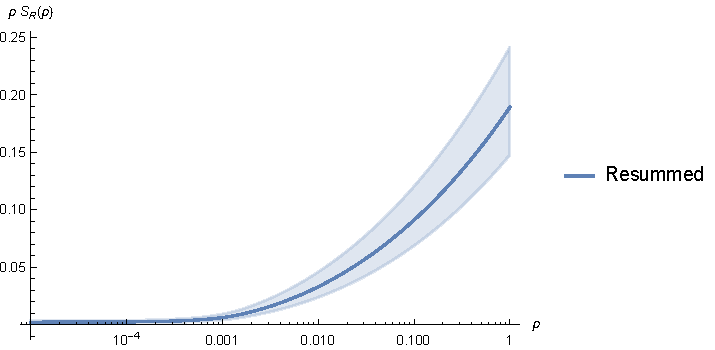
\includegraphics[width=0.9\textwidth]{figures/resummation_plot.pdf}

		\caption{\label{all-fig:resummed result}NLL resummed distribution of the soft function $S_R(\rho_s)$, from Eq.~\ref{all-eq:NLL soft function}. The top figure is the full range of $\rho_s$, while the bottom is zoomed in for small values of $\rho_s$. The running of $\alpha_s$ is fixed at the $Z$ boson mass, $\alpha_s(\SI{91.2}{\giga\electronvolt}) = 0.118$, from \cite{particle_data_group_review_2020}. The running is fixed below \SI{1}{\giga\electronvolt} in order to avoid the Landau pole at \SI{246}{\mega\electronvolt} \cite{larkoski_elementary_2019-1}. Uncertainty is estimated by varying $\mu$ within $\mu = \xi Q$ for $\xi \in [1/2, 2]$.}
	\end{center}
	\end{figure}

	On its own, the soft function $S_R$ does not have any physical meaning --- this much is clear from the manifest dependence on the arbitrary energy scale $\mu$. Physical meaning comes only in the context of the full cross section of Eq.~\ref{all-eq:full resummed result}, where we would expect to find (and, in fact, we would require) that all $\mu$-dependence cancel.\footnote{This cancellation is a strong cross-check to determine whether we have performed the calculation correctly.} Unfortunately, this means that until the entire distribution has been calculated, there is little we can do to satisfactorily convince ourselves that Eq.~\ref{all-eq:resummed inverse Laplace transform} is correct. The fact that Fig.~\ref{all-fig:resummed result} looks reasonable (i.e., it is smooth and continuous, and the uncertainty is not massive) is, however, a good start.


% \ifstandalone
% \bibliographystyle{../bsts/JHEP} 
% \bibliography{../jet_substructure}
% \fi
\end{document}

	

\chapter*{Conclusion}
     \addcontentsline{toc}{chapter}{Conclusion}
\chaptermark{Conclusion}
\markboth{Conclusion}{Conclusion}
\setcounter{chapter}{4}
\setcounter{section}{0}
	
	Conclusion here 


%If you feel it necessary to include an appendix, it goes here.
    % \appendix
    %   \chapter{The First Appendix}
    %   \chapter{The Second Appendix, for Fun}


%This is where endnotes are supposed to go, if you have them.
%I have no idea how endnotes work with LaTeX.

  \backmatter % backmatter makes the index and bibliography appear properly in the t.o.c...

% if you're using bibtex, the next line forces every entry in the bibtex file to be included
% in your bibliography, regardless of whether or not you've cited it in the thesis.
    % \nocite{*}

% Rename my bibliography to be called "Works Cited" and not "References" or ``Bibliography''
% \renewcommand{\bibname}{Works Cited}

%    \bibliographystyle{bsts/mla-good} % there are a variety of styles available; 
%  \bibliographystyle{plainnat}
% replace ``plainnat'' with the style of choice. You can refer to files in the bsts or APA 
% subfolder, e.g. 
 \bibliographystyle{bsts/myJHEP}  % or
 \bibliography{jet_substructure}
 % Comment the above two lines and uncomment the next line to use biblatex-chicago.
 %\printbibliography[heading=bibintoc]

% Finally, an index would go here... but it is also optional.
\end{document}
